% ============================================================
%  Science Skills and Safety — Experiment Booklet (one section per experiment)
%  Year 7 (Year 8 extension)  |  Victorian Curriculum F–10 Version 2.0
%  Compile with: xelatex three times, then python3 fill.py Science_Skills_Experiment_Booklet_Yr7
% ============================================================
\documentclass[11pt,a4paper]{article}

% ── Fonts (compile with LuaLaTeX) ────────────────────────────────────────────
\usepackage{fontspec}
% Bundled fonts (in ./fonts/) so the document compiles anywhere with XeLaTeX/LuaLaTeX
\setmainfont{Lato}[                   % body — humanist sans (stands in for deck's Inter)
  Path=./fonts/, Extension=.ttf, Ligatures=TeX,
  UprightFont=Lato-Regular, ItalicFont=Lato-Italic,
  BoldFont=Lato-Bold, BoldItalicFont=Lato-BoldItalic ]
\newfontfamily\headingfont{Poppins}[  % display/headings — matches the slide decks
  Path=./fonts/, Extension=.ttf, Ligatures=TeX,
  UprightFont=Poppins-Regular, ItalicFont=Poppins-Italic,
  BoldFont=Poppins-Bold, BoldItalicFont=Poppins-BoldItalic ]
\setlength{\headheight}{22pt}

\usepackage[protrusion=true,expansion=false]{microtype}
\usepackage[a4paper, top=2cm, bottom=2cm, left=2cm, right=2cm]{geometry}
\usepackage{xcolor}
\usepackage{tikz}
\usetikzlibrary{arrows.meta, shapes.geometric, calc, positioning, decorations.pathreplacing}
\usepackage{tcolorbox}
\tcbuselibrary{skins, breakable, raster}
\usepackage{fancyhdr}
\usepackage{titlesec}
\usepackage{enumitem}
\usepackage{booktabs}
\usepackage{tabularx}
\usepackage{array}
\usepackage{colortbl}
\usepackage{multicol}
\usepackage{amsmath}
\usepackage{needspace}
% TikZ diagram macros are embedded below (just before \begin{document}) for easy editing.
\usepackage{longtable}
\usepackage{lastpage}
\usepackage{calc}
\usepackage{mdframed}
\usepackage{setspace}
\usepackage{ragged2e}
% PDF bookmarks: one per lesson (made in \sectiondiv) plus the cover and
% contents, and links from the contents table to each lesson.
% implicit=false: hyperref adds no anchors of its own (an anchor on each
% list item nudged lists down 1.5 mm, which would undo the page fill).
% hidelinks keeps the links invisible, so the printed pages are unchanged.
\usepackage[implicit=false, hidelinks,
  pdftitle={Science Skills and Safety — Experiment Booklet},
  pdfsubject={Years 7–8 Science, Victorian Curriculum F–10 v2.0}]{hyperref}
\usepackage{bookmark} % writes the outline itself, which implicit=false switches off in hyperref
% hyperref 7.01 with implicit=false leaves \Hy@PageAnchorSlide undefined, which
% throws at \end{document} and stops fill.py (it builds with -halt-on-error).
\makeatletter\providecommand\Hy@PageAnchorSlide{}\makeatother

% ── Colour Palette ───────────────────────────────────────────────────────────
% Remapped to the slide-deck palette (names kept so body + diagrams cascade)
\definecolor{NavyBlue}   {HTML}{16305C}
\definecolor{MidBlue}    {HTML}{2E6FE0}
\definecolor{LightBlue}  {HTML}{E8F1FF}
\definecolor{TealGreen}  {HTML}{0F6E63}
\definecolor{LightGreen} {HTML}{E0F7F3}
\definecolor{GoldDark}   {HTML}{C77F12}
\definecolor{GoldLight}  {HTML}{FFF3DC}
\definecolor{PurpleDark} {HTML}{5B3FC0}
\definecolor{PurpleLight}{HTML}{EFE9FF}
\definecolor{OrangeDark} {HTML}{C9483D}
\definecolor{OrangeLight}{HTML}{FFE9E6}
\definecolor{MidGrey}    {HTML}{AEBED4}
\definecolor{LightGrey}  {HTML}{F2F5FA}
\definecolor{DarkGrey}   {HTML}{3A4759}
\definecolor{TableHead}  {HTML}{16305C}
\definecolor{RowAlt}     {HTML}{EEF4FF}
% Bright accent tints (deck) for bars, rules and chips
\definecolor{Blue}   {HTML}{2E6FE0}
\definecolor{Teal}   {HTML}{18A999}
\definecolor{Amber}  {HTML}{F5A623}
\definecolor{Coral}  {HTML}{FF6B5E}
\definecolor{Violet} {HTML}{7C5CE0}
\definecolor{Sky}    {HTML}{4DA3FF}
\definecolor{Ink}    {HTML}{16223A}
\definecolor{Line}   {HTML}{DDE5F0}
\definecolor{Paper}  {HTML}{FBFCFE}

% ── Page Style ───────────────────────────────────────────────────────────────
\pagestyle{fancy}
\fancyhf{}
\renewcommand{\headrulewidth}{0.4pt}
\renewcommand{\headrule}{\hbox to\headwidth{\color{NavyBlue}\leaders\hrule height \headrulewidth\hfill}}
\fancyhead[L]{\headingfont\small\color{NavyBlue}Science Skills and Safety \textbar{} Experiment Booklet}
\fancyhead[R]{\headingfont\small\color{DarkGrey}Year 7 \textbar{} Victorian Curriculum F--10 v2.0}
\fancyfoot[C]{\headingfont\small\color{DarkGrey}\thepage\ \textbar{} \pageref{LastPage}}
\fancypagestyle{plain}{%
  \fancyhf{}
  \fancyfoot[C]{\headingfont\small\color{DarkGrey}\thepage\ \textbar{} \pageref{LastPage}}
  \renewcommand{\headrulewidth}{0pt}
}

% ── Section Formatting ───────────────────────────────────────────────────────
\titleformat{\section}
  {\headingfont\color{NavyBlue}\Large\bfseries}
  {}{0em}{}
  [{\color{Teal}\rule[0.6ex]{2.2em}{3pt}}{\color{Line}\rule[0.6ex]{\dimexpr\linewidth-2.2em\relax}{1pt}}]
\titlespacing{\section}{0pt}{18pt}{8pt}

\titleformat{\subsection}
  {\headingfont\color{MidBlue}\large\bfseries}
  {\thesubsection}{0.6em}{}
\titlespacing{\subsection}{0pt}{12pt}{4pt}

\titleformat{\subsubsection}
  {\headingfont\color{NavyBlue}\normalsize\bfseries}
  {}{0em}{}
\titlespacing{\subsubsection}{0pt}{8pt}{2pt}

% Deck-style eyebrow / kicker (optional use)
\newcommand{\kicker}[2][Teal]{%
  {\headingfont\bfseries\footnotesize\color{#1}%
   \textcolor{#1}{\rule[0.18ex]{1.6em}{2.2pt}}\hspace{0.5em}\MakeUppercase{#2}\par}%
  \vspace{2pt}}

% ── Custom tcolorbox Environments ────────────────────────────────────────────

% Section divider banner
\newtcolorbox{sectionbanner}[2]{
  enhanced, breakable=false,
  colback=NavyBlue, colframe=NavyBlue,
  fontupper=\color{white}\bfseries\large,
  left=4mm, right=4mm, top=3mm, bottom=3mm,
  title={\color{white}\Huge\bfseries #1},
  attach boxed title to top left={yshift=-2mm, xshift=4mm},
  boxed title style={colback=NavyBlue, colframe=NavyBlue},
  after upper={\par\smallskip\normalfont\normalsize\color{white!80!NavyBlue}\textit{#2}}
}

% Key info box (blue)
\newtcolorbox{infobox}[1]{
  breakable, arc=2.5mm, boxrule=0.5pt,
  colback=LightBlue, colframe=Blue!40,
  fonttitle=\headingfont\bfseries, coltitle=MidBlue,
  title={#1},
  left=4mm, right=3.5mm, top=2.5mm, bottom=2.5mm
}

% Scaffold box (yellow)
\newtcolorbox{scaffold}[1]{
  breakable, arc=2.5mm, boxrule=0.5pt,
  colback=GoldLight, colframe=Amber!40,
  fonttitle=\headingfont\bfseries, coltitle=GoldDark,
  title={#1},
  left=4mm, right=3.5mm, top=2.5mm, bottom=2.5mm
}

% Worked example box
\newtcolorbox{workedexbox}[1]{
  breakable, arc=2.5mm, boxrule=0.5pt,
  colback=white, colframe=Amber!50,
  fonttitle=\headingfont\bfseries, coltitle=GoldDark,
  title={#1},
  left=4mm, right=3.5mm, top=2.5mm, bottom=2.5mm
}
% Worked examples: \begin{workedex}{title} -> "Worked Example N.M --- title",
% auto-numbered per section and labelled we:N.M. Never type the number.
\newcounter{wenum}[section]
\renewcommand{\thewenum}{\thesection.\arabic{wenum}}
\newenvironment{workedex}[1]
  {\refstepcounter{wenum}\label{we:\thewenum}\begin{workedexbox}{Worked Example \thewenum\ --- #1}}
  {\end{workedexbox}}

% We do: straight after each worked example, a near-identical question the
% class works through together, with its own writing space. Numbered to
% match the worked example above it and labelled wd:N.M.
%   \begin{wedo}{title} question ... \answerbox{h} \end{wedo}
\newtcolorbox{wedobox}[1]{
  enhanced, breakable=false, arc=2.5mm, boxrule=0.5pt,
  colback=white, colframe=TealGreen!55,
  fonttitle=\headingfont\bfseries, coltitle=TealGreen!75!black,
  title={#1},
  left=4mm, right=3.5mm, top=2.5mm, bottom=2.5mm
}
\newenvironment{wedo}[1]
  {\par\needspace{9\baselineskip}\begin{wedobox}{We do \thewenum\ --- #1}\label{wd:\thewenum}\ignorespaces}
  {\end{wedobox}}

% Year 7 box (blue)
\newtcolorbox{yr7box}{
  breakable, arc=2.5mm, boxrule=0.5pt,
  colback=LightBlue, colframe=Blue!40,
  left=4mm, right=3.5mm, top=2.5mm, bottom=2.5mm
}

% Year 8 extension box (violet)
\newtcolorbox{yr8box}{
  breakable, arc=2.5mm, boxrule=0.5pt,
  colback=PurpleLight, colframe=Violet!40,
  left=4mm, right=3.5mm, top=2.5mm, bottom=2.5mm
}

% Answer lines box
\newcommand{\answerbox}[1]{%
  \begin{tcolorbox}[
    enhanced, breakable, arc=2mm,
    colback=Paper, colframe=Line,
    left=2mm, right=2mm, top=1mm, bottom=1mm,
    boxrule=1pt,
    height=#1
  ]
  \end{tcolorbox}%
}

% Experiment header
\newtcolorbox{expheader}[3]{
  breakable=false, arc=2.5mm,
  colback=RowAlt, colframe=Amber!50, boxrule=0.5pt,
  fonttitle=\headingfont\bfseries\large, coltitle=NavyBlue,
  title={Experiment #1: #2},
  left=4mm, right=3.5mm, top=2.5mm, bottom=2.5mm,
  after upper={\par\smallskip
    {\headingfont\bfseries\color{GoldDark}Aim:}\ \textit{#3}},
}

% Reading comprehension passage box (green)
\newtcolorbox{readingbox}[1]{
  breakable, arc=2.5mm, boxrule=0.5pt,
  colback=white, colframe=Teal!50,
  fonttitle=\headingfont\bfseries, coltitle=TealGreen,
  title={#1},
  left=4mm, right=3.5mm, top=2.5mm, bottom=2.5mm,
  fontupper=\normalsize
}

% Skill-builder box (for beginner scaffolding)
\newtcolorbox{skillbox}[1]{
  breakable, arc=2.5mm, boxrule=0.5pt,
  colback=RowAlt, colframe=Blue!40,
  fonttitle=\headingfont\bfseries, coltitle=MidBlue,
  title={#1},
  left=4mm, right=3.5mm, top=2.5mm, bottom=2.5mm
}

% ── Custom Commands ───────────────────────────────────────────────────────────

% Question: \question{marks}{text}  (marks can be empty)
% Numbered automatically as Q<section>.<n>, reset every section.
% Do NOT write numbers by hand.
\newcounter{qnum}[section]
\renewcommand{\theqnum}{\thesection.\arabic{qnum}}
\newcommand{\question}[2]{%
  \refstepcounter{qnum}%
  \needspace{3\baselineskip}%
  \medskip
  \noindent\label{q:\theqnum}\textbf{Q\theqnum}\ifx&#1&\else\ \textcolor{DarkGrey}{(#1 mark\ifnum#1=1\else s\fi)}\fi\quad #2%
  \medskip
}

% Inline marks note
\newcommand{\markscount}[1]{\hfill\textcolor{DarkGrey}{\textit{(#1 mark\ifnum#1=1\else s\fi)}}}

% ── Practice set counter and question macros ─────────────────────────────────
\newcounter{pqnum}
\newcommand{\practiceset}[1]{%
  \needspace{6\baselineskip}
  \setcounter{pqnum}{0}%
  \vspace{6pt}
  {\headingfont\bfseries\large\color{GoldDark} Practice Set --- #1}\\[-2pt]
  {\color{Amber}\rule{\linewidth}{1pt}}\\[2pt]
}
% \pq{question text}{working box height}
\newcommand{\pq}[2]{%
  \stepcounter{pqnum}%
  \needspace{4\baselineskip}
  \vspace{5pt}
  \noindent\textbf{\thepqnum.}\quad #1\par
  \vspace{2pt}
  \answerbox{#2}
}
% Two short questions side by side, each with its own box
\newcommand{\pqpair}[4]{%
  \needspace{4\baselineskip}
  \vspace{5pt}
  \noindent
  \begin{minipage}[t]{0.48\linewidth}
    \stepcounter{pqnum}\textbf{\thepqnum.}\quad #1\par\vspace{2pt}
    \begin{tcolorbox}[enhanced,arc=2mm,colback=Paper,colframe=Line,left=2mm,right=2mm,
      top=1mm,bottom=1mm,boxrule=1pt,height=#2]\end{tcolorbox}
  \end{minipage}\hfill
  \begin{minipage}[t]{0.48\linewidth}
    \stepcounter{pqnum}\textbf{\thepqnum.}\quad #3\par\vspace{2pt}
    \begin{tcolorbox}[enhanced,arc=2mm,colback=Paper,colframe=Line,left=2mm,right=2mm,
      top=1mm,bottom=1mm,boxrule=1pt,height=#4]\end{tcolorbox}
  \end{minipage}
}

% ── Comprehension question macro (compact, lined) ────────────────────────────
\newcounter{rcnum}
\newcommand{\rcreset}{\setcounter{rcnum}{0}}
\newcommand{\rcq}[2]{%
  \stepcounter{rcnum}%
  \needspace{3\baselineskip}
  \vspace{4pt}
  \noindent\textbf{C\thercnum.}\quad #1\par
  \vspace{2pt}
  \linedbox{#2}
}

% Section divider (big numbered banner): \sectiondiv{title}{summary}
%
% This IS the section: it steps the real section counter, so subsections,
% tasks, questions and figures inside it are numbered N.M automatically.
% Put \label{sec:N} straight after it. Never hand-type a section number.
\newcommand{\sectiondiv}[2]{%
  \needspace{5\baselineskip}%
  \refstepcounter{section}%
  % PDF bookmark for the lesson; its anchor, lesson.N.1, is what the contents table links to
  \pdfbookmark[1]{Lesson \thesection{} — #1}{lesson.\thesection}%
  \begin{tcolorbox}[
    enhanced, breakable=false, arc=3.5mm,
    colback=NavyBlue, colframe=NavyBlue, boxrule=0pt,
    sidebyside, sidebyside align=center,
    lefthand width=2.4cm,
    left=2mm, right=4mm, top=4mm, bottom=4mm
  ]
    \begin{center}
      {\headingfont\bfseries\color{white!35!NavyBlue}\fontsize{50}{50}\selectfont \thesection}
    \end{center}
    \tcblower
    {\headingfont\bfseries\color{white}\LARGE #1}\\[3pt]
    {\itshape\color{white!75!NavyBlue}\small #2}
  \end{tcolorbox}%
}

% Tasks: \task, \task[a] (part a of a NEW task), \taskpart{b} (next part
% of the same task), \exttask (Year 8 "Extension" — same counter).
% Numbered Task <section>.<n>, reset every section. Do NOT type numbers.
% Every task, question and figure also gets an automatic label
% (task:1.7b, q:2.4, fig:1.2, fig:E2.1) so page refs come from the .aux.
\newcounter{tasknum}[section]
\renewcommand{\thetasknum}{\thesection.\arabic{tasknum}}
\NewDocumentCommand{\task}{o}{\refstepcounter{tasknum}\label{task:\thetasknum\IfValueT{#1}{#1}}\textbf{Task \thetasknum\IfValueT{#1}{#1}}}
\newcommand{\taskpart}[1]{\label{task:\thetasknum#1}\textbf{Task \thetasknum#1}}
\newcommand{\exttask}{\refstepcounter{tasknum}\label{task:\thetasknum}\textbf{Extension \thetasknum}}

% Figure captions: \figcap[fig:label]{caption} -> "Figure N.M --- caption"
% \expfigcap{caption} -> "Figure EN.M" (experiment pages). Both auto-numbered.
\newcounter{fignum}[section]
\renewcommand{\thefignum}{\thesection.\arabic{fignum}}
\newcounter{expfignum}[section]
\renewcommand{\theexpfignum}{E\thesection.\arabic{expfignum}}
\newcommand{\figcap}[2][]{%
  \begin{center}
    \refstepcounter{fignum}\label{fig:\thefignum}\if\relax\detokenize{#1}\relax\else\label{#1}\fi
    \small\itshape\color{DarkGrey} Figure \thefignum\ --- #2
  \end{center}%
}
\newcommand{\expfigcap}[1]{%
  \begin{center}
    \refstepcounter{expfignum}\label{fig:\theexpfignum}%
    \small\itshape\color{DarkGrey} Figure \theexpfignum\ --- #1
  \end{center}%
}

% Diagram include
\newcommand{\diagramfig}[3]{%  {filename}{width fraction}{caption}
  \begin{center}
    \includegraphics[width=#2\linewidth]{#1}\\[4pt]
    \small\itshape\color{DarkGrey} #3
  \end{center}%
}

% Table column types
\newcolumntype{L}[1]{>{\RaggedRight\arraybackslash}p{#1}}
\newcolumntype{C}[1]{>{\Centering\arraybackslash}p{#1}}

% Table header colour
\newcommand{\thead}[1]{\cellcolor{TableHead}\color{white}\bfseries #1}
\newcommand{\talt}{\rowcolor{RowAlt}}
\newcommand{\tmid}{\rowcolor{MidGrey}}

% Inline year tags
\newcommand{\tagyr}[1]{%
  \tikz[baseline=-0.5ex]\node[
    rounded corners=2pt,
    fill=#1!20, draw=#1, text=#1,
    inner xsep=4pt, inner ysep=1pt,
    font=\scriptsize\bfseries
  ]{Yr #1 only};}

% Draw answer lines
\newcommand{\anslines}[1]{%
  \vspace{2pt}%
  \foreach \n in {1,...,#1}{%
    \par\noindent\rule{\linewidth}{0.3pt}\vspace{3pt}%
  }%
}

% ── Document ─────────────────────────────────────────────────────────────────
% ── Optional-lesson note, shown under the lesson banner ──────────────────────
\newcommand{\optionalnote}[1]{%
  % the title is a bold lead-in on the first line rather than a title bar,
  % which keeps Lesson 11's reading on the lesson's first page
  \begin{tcolorbox}[enhanced, breakable=false, arc=2.5mm, boxrule=0.5pt,
    colback=PurpleLight, colframe=Violet!50,
    left=4mm, right=3.5mm, top=2mm, bottom=2mm]
  {\headingfont\bfseries\color{PurpleDark}Optional lesson \textbullet{} Year 8 extension.}\enspace #1
  \end{tcolorbox}\vspace{2pt}}


% ══════════════════════════════════════════════════════════════════════════════
%  LESSON STRUCTURE (lesson booklet, Oct 2026)
%  Every lesson runs in the same four parts, in this order:
%    \lessonpart{A}{Reading and comprehension}{Teal}   \label{read:N}
%    \lessonpart{B}{Theory and examples}{Blue}         \label{theory:N}
%    \lessonpart{C}{Practice}{Amber}                    \label{prac:N}
%    \lessonpart{D}{Above level}{Violet}                \label{ext:N}
%  Above-level / higher-order questions live ONLY in Part D, at the end.
% ══════════════════════════════════════════════════════════════════════════════
\newcommand{\lessonpart}[3]{%
  \par\if#1A\needspace{10\baselineskip}\vspace{10pt}\else
    \if#1C\notesfill\fi\clearpage\fi
  \begin{tcolorbox}[enhanced, breakable=false, arc=2mm, boxrule=0pt,
    colback=#3!14, borderline west={4pt}{0pt}{#3},
    left=4mm, right=3mm, top=1.6mm, bottom=1.6mm]
  {\headingfont\bfseries\color{#3!60!black}\large Part #1 \textbullet{} #2}
  \end{tcolorbox}\vspace{2pt}}

% Key vocabulary at the start of each lesson: students copy each definition
% from the vocabulary slide in the lesson's starter. First row = red scaffold.
\newcommand{\vocabhead}{%
  \par\vspace{6pt}%
  \begin{tcolorbox}[enhanced, breakable=false, arc=2mm, boxrule=0pt,
    colback=NavyBlue!10, borderline west={4pt}{0pt}{NavyBlue},
    left=4mm, right=3mm, top=1.6mm, bottom=1.6mm]
  {\headingfont\bfseries\color{NavyBlue}\large Key vocabulary}
  \end{tcolorbox}\vspace{2pt}%
  \noindent Copy the definition of each word from the slide. The first one has been done for you.\par}

% Curriculum codes under a lesson banner
\newcommand{\lessoncodes}[1]{%
  {\small\headingfont\color{DarkGrey}Victorian Curriculum 2.0:\ \textbf{#1}}\par\vspace{4pt}}

% Two short tasks side by side, each with its own working box
% \taskpair{text}{box height}{text}{box height}
% The two boxes line up: the shorter question is padded by the difference in
% text height (measured in a scratch box, task counter restored, no label).
\newsavebox\tpbox
\newlength\tpA \newlength\tpB
\newcount\tpsaved
\newcommand\tpmeasure[2]{%
  \tpsaved=\value{tasknum}%
  \sbox\tpbox{\vbox{\hsize=0.485\linewidth \linewidth=\hsize \parskip=0pt
    \renewcommand\label[1]{}\task #1\par}}%
  \setlength{#2}{\dimexpr\ht\tpbox+\dp\tpbox\relax}%
  \setcounter{tasknum}{\tpsaved}}
\newcommand{\taskpair}[4]{%
  \par\needspace{9\baselineskip}\vspace{4pt}%
  \tpmeasure{#1}{\tpA}\tpmeasure{#3}{\tpB}%
  \noindent
  \edef\abgrp{\number\numexpr\value{abox}+1\relax}%
  \begin{minipage}[t]{0.485\linewidth}
    \task #1\par\ifdim\tpB>\tpA\vspace{\dimexpr\tpB-\tpA\relax}\fi\vspace{2pt}\answerbox{#2}
  \end{minipage}\hfill
  \begin{minipage}[t]{0.485\linewidth}
    \task #3\par\ifdim\tpA>\tpB\vspace{\dimexpr\tpA-\tpB\relax}\fi\vspace{2pt}\answerbox{#4}
  \end{minipage}\par\gdef\abgrp{0}\vspace{4pt}}
% Two parts of one question side by side, with their answer boxes level:
% \ptpair{a}{part (a) text}{box height}{b}{part (b) text}{box height}.
% The shorter part's text gets space below it to match the longer one.
\newcommand\ptmeasure[3]{%
  \sbox\tpbox{\vbox{\hsize=0.485\linewidth \linewidth=\hsize \parskip=0pt \pt{#1}#2\par}}%
  \setlength{#3}{\dimexpr\ht\tpbox+\dp\tpbox\relax}}
\newcommand{\ptpair}[6]{%
  \ptmeasure{#1}{#2}{\tpA}\ptmeasure{#4}{#5}{\tpB}%
  \par\noindent
  \edef\abgrp{\number\numexpr\value{abox}+1\relax}%
  \begin{minipage}[t]{0.485\linewidth}
    \pt{#1}#2\par\ifdim\tpB>\tpA\vspace{\dimexpr\tpB-\tpA\relax}\fi\answerbox{#3}
  \end{minipage}\hfill
  \begin{minipage}[t]{0.485\linewidth}
    \pt{#4}#5\par\ifdim\tpA>\tpB\vspace{\dimexpr\tpA-\tpB\relax}\fi\answerbox{#6}
  \end{minipage}\par\gdef\abgrp{0}}

% Answer boxes never split across a page (a half box on its own page is useless)
% ── Page filling ────────────────────────────────────────────────────────────
% Every writing box gets an id. Its page is logged to \jobname.abp; fill.py
% measures the empty space left at the foot of each page and shares it out
% among that page's boxes via \jobname.abx (\abset{id}{extra}). Side-by-side
% boxes share a group so they grow together.
\newcounter{abox}
\newwrite\abpos \immediate\openout\abpos=\jobname.abp
\newcommand{\abset}[2]{\expandafter\gdef\csname abx@#1\endcsname{#2}}
\InputIfFileExists{\jobname.abx}{}{}
\def\abgrp{0}
\newcommand{\abnext}{\stepcounter{abox}%
  \edef\abcur{\ifcsname abx@\theabox\endcsname\csname abx@\theabox\endcsname\else 0pt\fi}}
\newcommand{\ablog}{\edef\abtmp{\noexpand\write\abpos{\theabox\space\abgrp\space\noexpand\thepage}}\abtmp}
\newcommand{\abh}[1]{\dimexpr#1+\abcur\relax}
\renewcommand{\answerbox}[1]{%
  \abnext
  \begin{tcolorbox}[enhanced, breakable=false, arc=2mm, colback=Paper, colframe=Line,
    left=2mm, right=2mm, top=1mm, bottom=1mm, boxrule=1pt, height=\abh{#1}]
  \end{tcolorbox}\ablog%
}
% \linedbox{height}: an answer box ruled in dotted thirds. Lines are \thirdrow/3 apart and run dotted, dotted,
% solid (the baseline), repeating, and end on one dotted line. The number of
% rows is worked out from the box's final height, so the ruling still fills the
% box after fill.py has grown it; the rows are centred in the box.
\newlength\thirdrow \setlength\thirdrow{9mm}
\tikzset{thirdsolid/.style={draw=DarkGrey!70, line width=0.5pt},
         thirddot/.style={draw=DarkGrey!70, line width=0.6pt, dash pattern=on 0.9pt off 1.6pt}}
\newlength\lbH \newlength\lbO \newcount\lbN
\newcommand{\linedbox}[1]{%
  \abnext
  % interior height = box height less the 1pt frame top and bottom
  \setlength\lbH{\dimexpr\abh{#1}-2pt\relax}%
  % whole rows that fit with at least 3 mm spare top and bottom (at least one)
  \lbN=\numexpr(\dimexpr\lbH-6mm-\thirdrow/2\relax)/\thirdrow\relax
  \ifnum\lbN<1 \lbN=1 \fi
  \setlength\lbO{\dimexpr(\lbH-\lbN\thirdrow)/2\relax}%
  \begin{tcolorbox}[enhanced, breakable=false, arc=2mm, colback=Paper, colframe=Line,
    left=2mm, right=2mm, top=1mm, bottom=1mm, boxrule=1pt, height=\abh{#1},
    underlay={\begin{tcbclipinterior}
      \foreach \i in {1,...,\the\lbN}{
        \draw[thirddot] ([xshift=3mm,yshift=-\lbO-(\i-1)*\thirdrow]interior.north west) -- ([xshift=-3mm,yshift=-\lbO-(\i-1)*\thirdrow]interior.north east);
        \draw[thirddot] ([xshift=3mm,yshift=-\lbO-(\i-1)*\thirdrow-\thirdrow/3]interior.north west) -- ([xshift=-3mm,yshift=-\lbO-(\i-1)*\thirdrow-\thirdrow/3]interior.north east);
        \draw[thirdsolid] ([xshift=3mm,yshift=-\lbO-(\i-1)*\thirdrow-2*\thirdrow/3]interior.north west) -- ([xshift=-3mm,yshift=-\lbO-(\i-1)*\thirdrow-2*\thirdrow/3]interior.north east);}
      \draw[thirddot] ([xshift=3mm,yshift=-\lbO-\lbN\thirdrow]interior.north west) -- ([xshift=-3mm,yshift=-\lbO-\lbN\thirdrow]interior.north east);
    \end{tcbclipinterior}}]
  \end{tcolorbox}\ablog%
}
% Every written-response box is ruled the same way (Part A comprehension, We do,
% Part C tasks and Part D extensions, including side-by-side pairs). Space for
% mathematical working uses \workbox{height} instead and stays plain, as do
% \drawbox and the write-in tables.
\let\workbox\answerbox   % plain box: mathematical working (calculations) stays unruled
\let\answerbox\linedbox
% \drawbox{height}{contents}: white box for a diagram or drawing
\newcommand{\drawbox}[2]{%
  \abnext
  \begin{tcolorbox}[colback=white, colframe=MidGrey, boxrule=0.5pt, height=\abh{#1}]#2\end{tcolorbox}\ablog}
% Notes box at the end of Part B: fills whatever is left of the page (if worth it)
\newcommand{\notesfill}{\par
  \ifdim\dimexpr\pagegoal-\pagetotal\relax>3.2cm
    \vspace*{\fill}%
    \begin{tcolorbox}[enhanced, breakable=false, arc=2mm, colback=Paper, colframe=Line,
      left=2mm, right=2mm, top=1mm, bottom=1mm, boxrule=1pt,
      height=\dimexpr\pagegoal-\pagetotal-1.0cm\relax]
      {\small\headingfont\color{DarkGrey}Notes}
    \end{tcolorbox}%
  \fi}



% Centred table: wrap every content table in \begin{ctab} ... \end{ctab}
% (figures already centre themselves inside their \diag... macros)
% ctab also registers write-in tables (S column) for page filling: the extra
% height is per row, logged with the row count.
\newenvironment{ctab}{\par\smallskip\begingroup\centering
  \abnext\let\tbcur\abcur\global\wtrows0 }{\par
  \ifnum\wtrows>0 \edef\abtmp{\noexpand\write\abpos{\theabox\space\abgrp\space\noexpand\thepage\space\the\wtrows}}\abtmp\fi
  \endgroup\smallskip}

% ── Booklet formatting rules (Oct 2026) ─────────────────────────────────────
% 1. No marks are shown anywhere in the booklet.
\renewcommand{\markscount}[1]{}
% 2. A task's heading sits on its own line; its text starts on the next
%    line, left aligned. Parts (a), (b)… each start a new line: use \pt{a}.
\RenewDocumentCommand{\task}{o}{\par\noindent\refstepcounter{tasknum}\label{task:\thetasknum\IfValueT{#1}{#1}}\textbf{Task \thetasknum\IfValueT{#1}{#1}}\par\nobreak\noindent\ignorespaces}
\renewcommand{\taskpart}[1]{\par\noindent\label{task:\thetasknum#1}\textbf{Task \thetasknum#1}\par\nobreak\noindent\ignorespaces}
\renewcommand{\exttask}{\par\noindent\refstepcounter{tasknum}\label{task:\thetasknum}\textbf{Extension \thetasknum}\par\nobreak\noindent\ignorespaces}
\newcommand{\pt}[1]{\par\noindent\textbf{(#1)}\ \ignorespaces}
% Workstation pages (Experiment 1): numbered method steps with a hanging
% indent, and a one-line safety reminder under the materials list.
\newcommand{\wsstep}[1]{\par\noindent\hangindent=1.6em\hangafter=1\makebox[1.6em][l]{\textbf{#1}}\ignorespaces}
\newcommand{\wssafety}[1]{\par\smallskip{\small\textcolor{ScaffoldRed}{\headingfont\bfseries Safety:}\ #1}\par}
% 3. Tables have vertical rules between columns and down both sides
%    (write | between and around the columns, e.g. {|L{3cm}|C{2cm}|}).
%    Keep the normal padding at the outer edges (no @{} there): colortbl paints
%    header colour one \tabcolsep past each edge, so trimming the padding makes
%    the header overhang the grid.
\arrayrulecolor{MidGrey}
\setlength{\arrayrulewidth}{0.6pt}
% 4. Write-in tables: W/Z are left/centred columns that centre text
%    vertically; put the S column first (see below).
\newcolumntype{W}[1]{>{\RaggedRight\arraybackslash}m{#1}}
\newcolumntype{Z}[1]{>{\Centering\arraybackslash}m{#1}}
\def\tbcur{0pt}
\newcount\wtrows
\newcommand{\wh}{\global\advance\wtrows1 \rule[\dimexpr-0.75cm-\tbcur/2\relax]{0pt}{\dimexpr1.5cm+\tbcur\relax}}
% S = zero-width first column that makes every row of a write-in table
% at least 1.5 cm tall with its text vertically centred. Start each data
% row with "&"; start the header row with "\hd &" so it stays slim.
\newif\ifnowh
\newcolumntype{S}{@{}>{}c<{\ifnowh\else\wh\fi\global\nowhfalse}@{\hspace{\tabcolsep}}}
\newcommand{\hd}{\global\nowhtrue}
% 5. The first row of a multi-row write-in table is a worked scaffold in red.
\definecolor{ScaffoldRed}{HTML}{C0392B}
\newcommand{\scaf}[1]{\textcolor{ScaffoldRed}{\itshape #1}}
% 6. Tables are a light grid (rules between rows and columns) on white —
%    row shading is off, because colortbl paints shading over column rules.
\renewcommand{\talt}{}
\renewcommand{\tmid}{}
% ══════════════════════════════════════════════════════════════════════════════
%  EXPERIMENT BOOKLET LAYER (Nov 2026)
%  From 2027 every Year 7 unit collects its experiments into one A4 experiment
%  booklet that puts the experimental techniques and skills first. Every skill
%  comes from the faculty Science Skills continuum (Years 7--8 column) and is
%  named the same way everywhere: a code (QP1, PC4, PA2 …) on a chip coloured by
%  its sub-strand. Copy this block into the next unit's experiment booklet.
%
%  Each experiment runs in the same order:
%    \experimentdiv{title}{summary}{lesson}\label{sec:N}
%    key vocabulary · learning intentions · \begin{skillsfocus}
%    \exppart*{Technique spotlight}{Blue}   (technique, worked example, We do)
%    \exppart{Plan and safety}{Teal}        (aim, prediction, variables, risks)
%    \exppart{Method}{Teal}
%    \exppart{Results}{Amber}
%    \exppart{Analysis and evaluation}{Coral}
%    \exppart{Skill check}{NavyBlue}
% ══════════════════════════════════════════════════════════════════════════════
\usetikzlibrary{arrows.meta,calc,positioning}
\usepackage{pifont}

\newenvironment{keepext}{\par\begin{tcolorbox}[blankest, breakable=false]}{\end{tcolorbox}\par}
% graph-paper box: \graphgrid{height}
\newcommand{\graphgrid}[1]{%
  \begin{tcolorbox}[enhanced, breakable=false, colback=white, colframe=MidGrey, boxrule=0.5pt, height=#1,
    underlay={\begin{tcbclipinterior}\draw[step=5mm, Line, very thin] (interior.south west) grid (interior.north east);
      \draw[step=1cm, MidGrey!70, thin] (interior.south west) grid (interior.north east);\end{tcbclipinterior}}]
  \end{tcolorbox}}

% ── Skills (faculty Science Skills continuum, Years 7–8) ─────────────────────
% \defskill{code}{name}{colour}{VC code}{what it means}
\makeatletter
\newcommand{\defskill}[5]{%
  \expandafter\gdef\csname sk@n@#1\endcsname{#2}%
  \expandafter\gdef\csname sk@c@#1\endcsname{#3}%
  \expandafter\gdef\csname sk@v@#1\endcsname{#4}%
  \expandafter\gdef\csname sk@d@#1\endcsname{#5}}
\newcommand{\skname}[1]{\csname sk@n@#1\endcsname}
\newcommand{\skcode}[1]{\csname sk@v@#1\endcsname}
\newcommand{\skdesc}[1]{\csname sk@d@#1\endcsname}
% \sk{PC4}: the chip — code and name on the sub-strand colour
\newcommand{\sk}[1]{%
  \edef\sk@col{\csname sk@c@#1\endcsname}%
  \tikz[baseline=(c.base)]\node[rounded corners=2.5pt, fill=\sk@col!16, draw=\sk@col, line width=0.6pt,
    text=\sk@col!55!black, inner xsep=4pt, inner ysep=2pt, font=\headingfont\bfseries\scriptsize]
    (c) {#1\,\textperiodcentered\,\skname{#1}};}
% \skr{PC4}: the chip flush right at the end of a paragraph; drops to its own line if it does not fit
\newcommand{\skr}[1]{\unskip\nobreak\hfill\penalty50\hskip1em\null\nobreak\hfill\sk{#1}}
% \skc{PC4}: the code alone, for tight table cells
\newcommand{\skc}[1]{%
  \edef\sk@col{\csname sk@c@#1\endcsname}%
  \tikz[baseline=(c.base)]\node[rounded corners=2.5pt, fill=\sk@col!16, draw=\sk@col, line width=0.6pt,
    text=\sk@col!55!black, inner xsep=3pt, inner ysep=2pt, font=\headingfont\bfseries\scriptsize]
    (c) {#1};}
\makeatother

% Questioning and predicting — VC2S8I01
\defskill{QP1}{Testable hypothesis}{Teal}{VC2S8I01}{A prediction that an experiment can test, written as \emph{If \dots\ then \dots\ because \dots}}
\defskill{QP2}{Formulate an aim}{Teal}{VC2S8I01}{One sentence saying what the experiment will find out: \emph{To find out how \dots\ affects \dots}}
% Planning and conducting — VC2S8I02, VC2S8I03
\defskill{PC1}{Plan and follow a method}{Blue}{VC2S8I02}{Follow numbered steps in order, so that someone else could repeat the experiment and get the same results (repeatable)}
\defskill{PC2}{Identify variables}{Blue}{VC2S8I02}{Name the independent variable (what you change), the dependent variable (what you measure) and the controlled variables (what you keep the same)}
\defskill{PC3}{Risks and safety}{Blue}{VC2S8I02}{Name each hazard, the risk it causes and the control that prevents it; follow the lab rules}
\defskill{PC4}{Precision}{Blue}{VC2S8I02}{Choose equipment with a fine enough scale, read it to its smallest division, and repeat measurements to see how closely they agree}
\defskill{PC5}{Ethics}{Blue}{VC2S8I02}{Treat people, living things, the environment and other people's data with respect}
\defskill{PC6}{Collect data and measure}{Blue}{VC2S8I02}{Take each measurement at the right time, with its unit, and record it straight away}
\defskill{PC7}{Use and select equipment}{Blue}{VC2S8I03}{Name each piece of equipment, use it correctly and choose the right piece for the job}
\defskill{PC8}{Use digital tools}{Blue}{VC2S8I03}{Use stopwatches, data loggers, sensors and spreadsheets to collect and record data}
% Processing, modelling and analysing — VC2S8I04, VC2S8I05
\defskill{PA1}{Tables}{GoldDark}{VC2S8I04}{Organise data in a ruled table, with the independent variable first and units in the column headings}
\defskill{PA2}{Graphing}{GoldDark}{VC2S8I04}{Draw the right type of graph with a title, labelled axes with units, even scales and accurate points}
\defskill{PA3}{Mathematical relationships}{GoldDark}{VC2S8I04}{Process data with calculations: differences, averages, rates and formulas}
\defskill{PA4}{Creating models}{GoldDark}{VC2S8I04}{Build a physical, drawn or mathematical model that represents something real}
\defskill{PA5}{Patterns and trends}{GoldDark}{VC2S8I05}{Describe how the dependent variable changes as the independent variable changes, quoting data}
\defskill{PA6}{Correlation and causality}{GoldDark}{VC2S8I05}{Say whether two variables change together, and whether there is evidence that one causes the other}
\defskill{PA7}{Identify anomalies}{GoldDark}{VC2S8I05}{Spot a result that does not fit the pattern and suggest why it happened}
\defskill{PA8}{Interpreting models}{GoldDark}{VC2S8I05}{Use a model to explain an observation, and say what the model shows well and what it leaves out}
% Evaluating — VC2S8I06, VC2S8I07
\defskill{EV1}{Results against hypothesis}{OrangeDark}{VC2S8I06}{Say whether the results support the hypothesis, quoting data as evidence}
\defskill{EV2}{Compare with known concepts}{OrangeDark}{VC2S8I06}{Compare your results with accepted values and scientific ideas}
\defskill{EV3}{Error sources}{OrangeDark}{VC2S8I06}{Name what could have made results less accurate or less precise, and suggest how to improve the method}
\defskill{EV4}{Quality of secondary sources}{OrangeDark}{VC2S8I07}{Judge whether information from a website, book or video can be trusted}
\defskill{EV5}{Questions for further investigation}{OrangeDark}{VC2S8I07}{Pose a new question that follows from your results}
% Communicating — VC2S8I08
\defskill{CO1}{Scientific writing}{PurpleDark}{VC2S8I08}{Write in the third person, legibly, with correct spelling and grammar, short and to the point, using scientific terms}
\defskill{CO2}{Presentation formats}{PurpleDark}{VC2S8I08}{Choose the right format to show findings: a table, graph, scientific diagram, poster, report or talk}

% Skills focus panel at the top of each experiment:
%   \begin{skillsfocus} \focus{PC4}{what you do with it here} … \end{skillsfocus}
\newtcolorbox{skillsfocus}{
  enhanced, breakable=false, arc=2.5mm, boxrule=0.6pt,
  colback=white, colframe=NavyBlue!55,
  fonttitle=\headingfont\bfseries, coltitle=white, colbacktitle=NavyBlue,
  title={Skills focus --- the science skills this experiment builds},
  left=4mm, right=3.5mm, top=2mm, bottom=2mm}
\newcommand{\focus}[2]{\par\noindent\makebox[1.25cm][l]{\skc{#1}}\parbox[t]{\dimexpr\linewidth-1.25cm\relax}{\small\textbf{\skname{#1}}\,---\,#2}\par\vspace{2pt}}

% Learning intentions panel: \begin{lipanel} \inquiryli{…} \understandli{…} \sclist{…} \end{lipanel}
\newtcolorbox{lipanel}{
  enhanced, breakable=false, arc=2.5mm, boxrule=0.5pt,
  colback=LightBlue, colframe=Blue!40,
  fonttitle=\headingfont\bfseries, coltitle=MidBlue, title={Learning intentions},
  left=4mm, right=3.5mm, top=2mm, bottom=2mm}
\newcommand{\inquiryli}[1]{\par\noindent{\headingfont\bfseries\color{NavyBlue}Science Inquiry:}\ #1\par\vspace{2pt}}
\newcommand{\understandli}[1]{\par\noindent{\headingfont\bfseries\color{NavyBlue}Science Understanding:}\ #1\par\vspace{2pt}}
\newcommand{\sctitle}{\par\noindent{\headingfont\bfseries\color{NavyBlue}Success criteria}\par}

% Technique spotlight: \begin{technique}{title}{PC4} … \end{technique}
\newtcolorbox{technique}[2]{
  enhanced, breakable, arc=2.5mm, boxrule=0.6pt,
  colback=white, colframe=Blue!55,
  fonttitle=\headingfont\bfseries, coltitle=MidBlue, colbacktitle=LightBlue,
  title={Technique: #1\hfill\sk{#2}},
  left=4mm, right=3.5mm, top=2.5mm, bottom=2.5mm}

% Experiment divider: \experimentdiv{title}{summary}{lesson number}
% Steps the section counter, so tasks, worked examples and figures are N.M.
\newcommand{\experimentdiv}[3]{%
  \clearpage
  \refstepcounter{section}%
  \pdfbookmark[1]{Experiment \thesection{} — #1}{exp.\thesection}%
  \begin{tcolorbox}[
    enhanced, breakable=false, arc=3.5mm,
    colback=NavyBlue, colframe=NavyBlue, boxrule=0pt,
    sidebyside, sidebyside align=center,
    lefthand width=2.6cm,
    left=2mm, right=4mm, top=4mm, bottom=4mm]
    \begin{center}
      {\headingfont\bfseries\color{white!60!NavyBlue}\scriptsize EXPERIMENT}\\[-2pt]
      {\headingfont\bfseries\color{white!35!NavyBlue}\fontsize{46}{46}\selectfont \thesection}
    \end{center}
    \tcblower
    {\headingfont\bfseries\color{white}\LARGE #1}\\[3pt]
    {\itshape\color{white!75!NavyBlue}\small #2}\\[3pt]
    {\headingfont\color{Sky}\footnotesize Lesson #3}
  \end{tcolorbox}%
}

% Part bar inside an experiment. \exppart{title}{colour} starts a new page
% (new parts always start on a new page); \exppart*{…}{…} follows straight on.
\NewDocumentCommand{\exppart}{s m m}{%
  \par\IfBooleanTF{#1}{\needspace{10\baselineskip}\vspace{8pt}}{\clearpage}%
  \begin{tcolorbox}[enhanced, breakable=false, arc=2mm, boxrule=0pt,
    colback=#3!14, borderline west={4pt}{0pt}{#3},
    left=4mm, right=3mm, top=1.6mm, bottom=1.6mm]
  {\headingfont\bfseries\color{#3!60!black}\large #2}
  \end{tcolorbox}\vspace{2pt}}

% Skill check at the end of each experiment: students tick one column per row.
%   \begin{skillcheck} \scrow{PC4}{I can …} … \end{skillcheck}
\newcommand{\tickbox}{\tikz[baseline=-0.6ex]\draw[DarkGrey, line width=0.7pt, rounded corners=1pt] (0,-0.17) rectangle (0.34,0.17);}
\newenvironment{skillcheck}{%
  \par\noindent Read each statement. Tick the column that best describes you \emph{today}.\par
  \begin{ctab}\renewcommand{\arraystretch}{1.25}%
  \begin{tabular}{|W{3.9cm}|W{7.0cm}|Z{1.45cm}|Z{1.45cm}|Z{1.45cm}|}
  \hline\thead{Skill} & \thead{Success criterion} & \thead{Not yet} & \thead{Nearly} & \thead{Got it} \\ \hline}
  {\end{tabular}\end{ctab}}
\newcommand{\scrow}[2]{\rule{0pt}{1.1cm}\skc{#1}\enspace{\small\skname{#1}} & #2 & \tickbox & \tickbox & \tickbox \\ \hline}

% Write-in label under a drawing: \nameline{label}
\newcommand{\nameline}[1]{\par\noindent{\small #1}\ \leaders\hbox{\rule[-2pt]{1pt}{0.4pt}}\hfill\null\par}

% ── Equipment drawn as scientific diagrams (2D, side-on, outline only) ──────
% Each \eq... macro draws at the origin inside a tikzpicture. \eqpic[scale]{\eqBeaker}
% puts one on its own. The same shapes are used everywhere, so the booklet
% models exactly the drawings students are asked to make.
\tikzset{
  eq/.style={line width=0.9pt, draw=Ink, line cap=round, line join=round},
  eqlab/.style={draw=Ink, line width=0.4pt},
  eqtext/.style={font=\footnotesize, text=Ink, inner sep=1.5pt},
}
\newcommand{\eqpic}[2][1]{\begin{tikzpicture}[scale=#1, baseline=(current bounding box.center)]#2\end{tikzpicture}}
\newcommand{\eqBeaker}{\draw[eq] (-0.22,2.62) -- (0,2.45) -- (0,0) -- (1.8,0) -- (1.8,2.5);}
\newcommand{\eqFlask}{\draw[eq] (0.62,2.9) -- (0.65,2.8) -- (0.65,1.9) -- (0,0) -- (1.9,0) -- (1.25,1.9) -- (1.25,2.8) -- (1.28,2.9);}
\newcommand{\eqTestTube}{\draw[eq] (-0.06,3.0) -- (0,2.9) -- (0,0.3) arc[start angle=180,end angle=360,radius=0.3] -- (0.6,2.9) -- (0.66,3.0);}
\newcommand{\eqCylinder}{%
  \draw[eq] (-0.15,3.6) -- (0,3.5) -- (0,0.15) (0.6,0.15) -- (0.6,3.5);
  \draw[eq] (-0.35,0) rectangle (0.95,0.15);
  \foreach \y in {0.6,1.1,...,3.2} \draw[Ink, line width=0.5pt] (0.6,\y) -- (0.4,\y);}
\newcommand{\eqFunnel}{\draw[eq] (0,2.2) -- (0.75,1.0) -- (0.75,0) (1.85,2.2) -- (1.1,1.0) -- (1.1,0);}
\newcommand{\eqBasin}{\draw[eq] (0,0.9) .. controls (0.15,0.02) and (2.25,0.02) .. (2.4,0.9);}
\newcommand{\eqTripod}{%
  \draw[eq] (-0.15,2.0) rectangle (2.55,2.12);
  \draw[eq] (0.25,2.0) -- (0,0) (2.15,2.0) -- (2.4,0) (1.2,2.0) -- (1.2,0.15);}
\newcommand{\eqBunsen}{%
  \draw[eq] (0,0) rectangle (1.6,0.22);
  \draw[eq] (0.58,0.85) -- (0.58,2.3) (1.02,0.85) -- (1.02,2.3);
  \draw[eq] (0.5,0.22) rectangle (1.1,0.85);
  \fill[Ink] (0.72,0.42) rectangle (0.88,0.62);
  \draw[eq] (-0.65,0.06) rectangle (0,0.16);}
\newcommand{\eqThermometer}{%
  \draw[eq] (0.25,0.25) circle (0.2);
  \draw[eq] (0.15,0.43) -- (0.15,3.9) arc[start angle=180,end angle=0,radius=0.1] -- (0.35,0.43);
  \draw[Ink, line width=1.3pt] (0.25,0.45) -- (0.25,1.9);}
\newcommand{\eqStand}{%
  \draw[eq] (0,0) rectangle (2.3,0.2);
  \draw[eq] (0.35,0.2) -- (0.35,4.0) (0.5,0.2) -- (0.5,4.0);
  \draw[eq] (0.25,2.75) rectangle (0.75,3.2);
  \draw[eq] (0.75,2.92) -- (1.6,2.92) (0.75,3.03) -- (1.6,3.03);
  \draw[eq] (1.6,2.7) -- (1.6,3.25) (1.6,2.7) -- (1.95,2.7) (1.6,3.25) -- (1.95,3.25);}
\newcommand{\eqWatchGlass}{\draw[eq] (0,0.35) .. controls (0.5,-0.05) and (1.7,-0.05) .. (2.2,0.35);}
\newcommand{\eqTongs}{%
  \draw[eq] (0,0.1) -- (2.0,0.45) .. controls (2.3,0.5) and (2.45,0.35) .. (2.6,0.15)
            (0,0.0) -- (2.0,-0.35) .. controls (2.3,-0.4) and (2.45,-0.25) .. (2.6,-0.05);}

% A label line from a point on a drawing to text at the side: \eqlab{(x,y)}{(tx,ty)}{text}
\newcommand{\eqlab}[3]{\draw[eqlab] #1 -- #2 node[eqtext, anchor=west] {#3};}
\newcommand{\eqlabl}[3]{\draw[eqlab] #1 -- #2 node[eqtext, anchor=east] {#3};}

% ── Reading scales ──────────────────────────────────────────────────────────
% \readcyl{lowest}{highest}{labelled step}{small divisions per label}{reading}
% A close-up of a measuring cylinder's scale, the water drawn to the reading:
% the bottom of the meniscus sits exactly on the reading.
\pgfkeys{/pgf/number format/.cd, fixed, precision=1}
\newcommand{\readcyl}[5]{%
\begin{tikzpicture}[baseline=(current bounding box.south)]
  \pgfmathsetmacro\rcH{5.0}
  \pgfmathsetmacro\rcY{(#5-#1)*\rcH/(#2-#1)}
  \pgfmathtruncatemacro\rcN{round((#2-#1)/#3*#4)}
  \fill[black!10] (0,-0.3) -- (0,\rcY+0.16) .. controls (0.45,\rcY-0.05) and (1.15,\rcY-0.05) .. (1.6,\rcY+0.16) -- (1.6,-0.3) -- cycle;
  \draw[Ink, line width=0.9pt] (0,\rcY+0.16) .. controls (0.45,\rcY-0.05) and (1.15,\rcY-0.05) .. (1.6,\rcY+0.16);
  \foreach \k in {0,...,\rcN}{
    \pgfmathsetmacro\yy{\k*\rcH/\rcN}
    \pgfmathtruncatemacro\ismaj{mod(\k,#4)==0 ? 1 : 0}
    \ifnum\ismaj=1
      \draw[Ink, line width=0.75pt] (0,\yy) -- (0.6,\yy);
      \pgfmathsetmacro\lv{#1+\k/#4*#3}
      \node[anchor=west, font=\scriptsize\bfseries, inner sep=1pt, fill=white, fill opacity=0.8, text opacity=1] at (0.66,\yy) {\pgfmathprintnumber{\lv}};
    \else
      \draw[Ink, line width=0.4pt] (0,\yy) -- (0.32,\yy);
    \fi}
  \draw[eq] (0,-0.3) -- (0,\rcH+0.35) (1.6,-0.3) -- (1.6,\rcH+0.35);
  \node[font=\scriptsize, anchor=north] at (0.8,-0.35) {scale in mL};
\end{tikzpicture}}
% \readtherm{lowest}{highest}{labelled step}{small divisions per label}{reading}
\newcommand{\readtherm}[5]{%
\begin{tikzpicture}[baseline=(current bounding box.south)]
  \pgfmathsetmacro\rtH{5.0}
  \pgfmathsetmacro\rtY{(#5-#1)*\rtH/(#2-#1)}
  \pgfmathtruncatemacro\rtN{round((#2-#1)/#3*#4)}
  \draw[eq, fill=white] (0,-0.45) circle (0.3);
  \fill[black!75] (0,-0.45) circle (0.22);
  \fill[black!75] (-0.07,-0.3) rectangle (0.07,\rtY);
  \draw[eq] (-0.16,-0.2) -- (-0.16,\rtH+0.3) arc[start angle=180,end angle=0,radius=0.16] -- (0.16,-0.2);
  \foreach \k in {0,...,\rtN}{
    \pgfmathsetmacro\yy{\k*\rtH/\rtN}
    \pgfmathtruncatemacro\ismaj{mod(\k,#4)==0 ? 1 : 0}
    \ifnum\ismaj=1
      \draw[Ink, line width=0.75pt] (0.25,\yy) -- (0.75,\yy);
      \pgfmathsetmacro\lv{#1+\k/#4*#3}
      \node[anchor=west, font=\scriptsize\bfseries, inner sep=1pt] at (0.8,\yy) {\pgfmathprintnumber{\lv}};
    \else
      \draw[Ink, line width=0.4pt] (0.25,\yy) -- (0.52,\yy);
    \fi}
  \node[font=\scriptsize, anchor=north] at (0.3,-0.8) {scale in \textdegree C};
\end{tikzpicture}}
% \balancefig{reading}: an electronic balance showing a reading
\newcommand{\balancefig}[1]{%
\begin{tikzpicture}[baseline=(current bounding box.south)]
  \draw[eq, rounded corners=3pt] (0,0) rectangle (4.2,1.35);
  \draw[eq] (1.9,1.35) -- (1.9,1.55) (2.3,1.35) -- (2.3,1.55);
  \draw[eq, rounded corners=1pt] (0.5,1.55) rectangle (3.7,1.72);
  \draw[eq, fill=LightGrey] (0.35,0.35) rectangle (2.75,1.02);
  \node[font=\headingfont\bfseries\large, anchor=east] at (2.65,0.68) {#1};
  \draw[eq] (3.3,0.68) circle (0.2);
  \node[font=\tiny\bfseries] at (3.3,0.3) {TARE};
\end{tikzpicture}}
% Bunsen burner with a flame: \bunsenflame{safety|heating}
\newcommand{\bunsenflame}[1]{%
\begin{tikzpicture}[baseline=(current bounding box.south)]
  \def\fl{#1}\def\safe{safety}%
  \ifx\fl\safe
    \fill[black!14] (0.8,2.3) .. controls (0.05,3.0) and (0.45,4.3) .. (0.85,5.0) .. controls (1.05,4.4) and (1.55,3.1) .. (0.8,2.3);
    \draw[Ink, line width=0.6pt] (0.8,2.3) .. controls (0.05,3.0) and (0.45,4.3) .. (0.85,5.0) .. controls (1.05,4.4) and (1.55,3.1) .. (0.8,2.3);
  \else
    \fill[white] (0.8,2.3) .. controls (0.45,2.8) and (0.6,3.5) .. (0.8,3.9) .. controls (1.0,3.5) and (1.15,2.8) .. (0.8,2.3);
    \draw[Ink, line width=0.6pt] (0.8,2.3) .. controls (0.45,2.8) and (0.6,3.5) .. (0.8,3.9) .. controls (1.0,3.5) and (1.15,2.8) .. (0.8,2.3);
    \fill[black!30] (0.8,2.3) .. controls (0.65,2.55) and (0.7,2.85) .. (0.8,3.0) .. controls (0.9,2.85) and (0.95,2.55) .. (0.8,2.3);
  \fi
  \draw[eq] (0,0) rectangle (1.6,0.22);
  \draw[eq] (0.58,0.85) -- (0.58,2.3) (1.02,0.85) -- (1.02,2.3);
  \draw[eq] (0.5,0.22) rectangle (1.1,0.85);
  \ifx\fl\safe\draw[Ink, line width=0.5pt, densely dotted] (0.72,0.42) rectangle (0.88,0.62);\else\fill[Ink] (0.72,0.42) rectangle (0.88,0.62);\fi
  \draw[eq] (-0.65,0.06) rectangle (0,0.16);
\end{tikzpicture}}
% ══════════════════════════════════════════════════════════════════════════════
%  2027 WORKBOOK STYLE (Year 7 workbook redesign, Nov 2026) — A4 version
%  The look of the A5 trial (space/booklet/a5-test) on an A4 page:
%    · colour cover from the unit's cover art, black-and-white inside
%    · headings in Outfit (the site's heading face), body in Lato
%    · each experiment opens with a band: number, title, ink symbol, heavy rule
%    · boxes told apart by frame and icon, never by colour:
%        I do ●  solid · We do ●● dashed · You do ●●● heavy
%        Key idea / technique ◆ thin · Above level ▲ double · Country ◎ dotted
%    · skill tags are ink tabs carrying the code (QP1, PC4 …) plus the name
%  Everything above this block still names the old colours; they are mapped to
%  ink here, so the body never needs to know which look it is printed in.
% ══════════════════════════════════════════════════════════════════════════════

\usetikzlibrary{patterns}
% ── Fonts ───────────────────────────────────────────────────────────────────
% Bold is Outfit SemiBold, the weight the site uses; Outfit has no italic,
% so a slanted one stands in.
\renewfontfamily\headingfont{Outfit}[
  Path=./fonts/, Extension=.ttf, Ligatures=TeX,
  UprightFont=Outfit-Regular, BoldFont=Outfit-SemiBold,
  ItalicFont=Outfit-Regular, ItalicFeatures={FakeSlant=0.18},
  BoldItalicFont=Outfit-SemiBold, BoldItalicFeatures={FakeSlant=0.18} ]

% ── Black and white inside ──────────────────────────────────────────────────
\definecolor{Ink}{HTML}{111111}
\colorlet{NavyBlue}{Ink}\colorlet{MidBlue}{Ink}\colorlet{TealGreen}{Ink}
\colorlet{GoldDark}{Ink}\colorlet{PurpleDark}{Ink}\colorlet{OrangeDark}{Ink}
\colorlet{TableHead}{Ink}
\colorlet{Blue}{Ink}\colorlet{Teal}{Ink}\colorlet{Amber}{Ink}\colorlet{Coral}{Ink}
\colorlet{Violet}{Ink}\colorlet{Sky}{Ink}
\colorlet{LightBlue}{white}\colorlet{LightGreen}{white}\colorlet{GoldLight}{white}
\colorlet{PurpleLight}{white}\colorlet{OrangeLight}{white}\colorlet{RowAlt}{white}
\colorlet{LightGrey}{white}\colorlet{Paper}{white}
\colorlet{DarkGrey}{black!72}\colorlet{MidGrey}{black!45}\colorlet{Line}{black!45}
\arrayrulecolor{black!60}

% ── Page style ──────────────────────────────────────────────────────────────
\fancypagestyle{fancy}{%
  \fancyhf{}%
  \renewcommand{\headrulewidth}{0.4pt}%
  \renewcommand{\headrule}{\hbox to\headwidth{\color{Ink}\leaders\hrule height \headrulewidth\hfill}}%
  \fancyhead[L]{\headingfont\footnotesize Science Skills and Safety \textbullet\ Experiment Booklet}%
  \fancyhead[R]{\headingfont\footnotesize\leftmark}%
  \fancyfoot[C]{\headingfont\footnotesize\thepage}}
\fancypagestyle{plain}{\fancyhf{}\renewcommand{\headrulewidth}{0pt}%
  \fancyfoot[C]{\headingfont\footnotesize\thepage}}
\fancypagestyle{opener}{\fancyhf{}\renewcommand{\headrulewidth}{0pt}%
  \fancyfoot[C]{\headingfont\footnotesize\thepage}}
\pagestyle{fancy}
\markboth{}{}

\titleformat{\subsubsection}{\headingfont\normalsize\bfseries}{}{0em}{}

% ── Box system: told apart by frame and icon, never by colour ───────────────
\newcommand{\icodots}[1]{\tikz[baseline=-0.6ex]{\foreach \k in {1,...,#1}{\fill[white] (\k*1.9mm,0) circle (0.7mm);}}}
\newcommand{\icokey}{\tikz[baseline=-0.6ex]{\fill[white] (0,0.9mm)--(0.9mm,0)--(0,-0.9mm)--(-0.9mm,0)--cycle;}}
\newcommand{\icoup}{\tikz[baseline=-0.6ex]{\fill[white] (-1mm,-0.8mm)--(1mm,-0.8mm)--(0,1mm)--cycle;}}
\newcommand{\icocountry}{\tikz[baseline=-0.6ex]{\draw[white,line width=0.5pt] (0,0) circle (1mm); \fill[white] (0,0) circle (0.45mm);}}
\newcommand{\icoskill}{\tikz[baseline=-0.6ex]{\fill[white] (-0.85mm,-0.85mm) rectangle (0.85mm,0.85mm);}}
\newcommand{\tagicon}[1]{\tikz[baseline=-0.6ex]\node[fill=Ink, rounded corners=0.8mm, inner xsep=1.2mm, inner ysep=1mm]{#1};}
\tcbset{wbbase/.style={enhanced, colback=white, arc=1.2mm,
    left=3.5mm, right=3.5mm, top=4.2mm, bottom=2.6mm, before skip=11pt, after skip=8pt,
    attach boxed title to top left={xshift=3mm, yshift=-2.4mm},
    boxed title style={colback=Ink, colframe=Ink, arc=0.8mm, boxrule=0pt,
                       left=1.6mm, right=1.8mm, top=0.6mm, bottom=0.6mm},
    fonttitle=\headingfont\bfseries\footnotesize, coltitle=white}}

% I do: the worked example (solid frame, one dot)
\renewtcolorbox{workedexbox}[1]{wbbase, breakable, colframe=Ink, boxrule=1pt,
  title={\icodots{1}\ I do \textbullet\ #1}}
\renewenvironment{workedex}[1]
  {\refstepcounter{wenum}\label{we:\thewenum}\begin{workedexbox}{Worked example \thewenum\ --- #1}}
  {\end{workedexbox}}
% We do: straight after its worked example (dashed frame, two dots)
\renewtcolorbox{wedobox}[1]{wbbase, breakable=false, frame hidden,
  borderline={1.1pt}{0pt}{Ink, dash pattern=on 4pt off 2.6pt},
  title={\icodots{2}\ #1}}
\renewenvironment{wedo}[1]
  {\par\begin{wedobox}{We do \thewenum\ --- #1}\label{wd:\thewenum}\ignorespaces}
  {\end{wedobox}}
% You do: a set of practice tasks on your own (heavy frame, three dots)
\newtcolorbox{youdobox}[1][Check your understanding]{wbbase, breakable=false,
  colframe=Ink, boxrule=2.4pt, top=5mm,
  title={\icodots{3}\ You do \textbullet\ #1}}
% Key idea, technique, safety, word banks (thin frame, diamond)
\renewtcolorbox{infobox}[1]{wbbase, breakable, colframe=Ink, boxrule=0.5pt,
  title={\icokey\ #1}}
\renewtcolorbox{scaffold}[1]{wbbase, breakable, colframe=Ink, boxrule=0.5pt,
  title={\icokey\ #1}}
\renewtcolorbox{technique}[2]{wbbase, breakable, colframe=Ink, boxrule=0.5pt,
  title={\icokey\ Technique \textbullet\ #1\enspace\textbar\enspace #2 \skname{#2}}}
% Above level (double frame, triangle)
\renewtcolorbox{yr8box}{wbbase, breakable, frame hidden,
  borderline={0.6pt}{0pt}{Ink}, borderline={0.6pt}{1.6pt}{Ink},
  title={\icoup\ Going further \textbullet\ Above level}}
% Country (dotted frame, ring)
\newtcolorbox{countrybox}[1]{wbbase, breakable, frame hidden,
  borderline={1.4pt}{0pt}{Ink, line cap=round, dash pattern=on 0pt off 2.4pt},
  title={\icocountry\ #1}}
% Learning intentions and skills focus (thin frame; square for skills)
\renewtcolorbox{lipanel}{wbbase, breakable=false, colframe=Ink, boxrule=0.5pt,
  title={\icokey\ Learning intentions}}
\renewtcolorbox{skillsfocus}{wbbase, breakable=false, colframe=Ink, boxrule=1pt,
  title={\icoskill\ Skills focus \textbullet\ the science skills this experiment builds},
  before upper={\begin{multicols}{2}\raggedcolumns}, after upper={\end{multicols}}}

% ── Skill tags: an ink tab with the code, then the name ─────────────────────
\makeatletter
\renewcommand{\skc}[1]{%
  \tikz[baseline=(c.base)]\node[rounded corners=0.8mm, fill=Ink, text=white, inner xsep=1.5mm, inner ysep=0.7mm,
    font=\headingfont\bfseries\scriptsize] (c) {#1};}
\renewcommand{\sk}[1]{\mbox{\skc{#1}\,{\headingfont\bfseries\footnotesize\skname{#1}}}}
\makeatother
\renewcommand{\focus}[2]{\par\noindent\makebox[1.1cm][l]{\skc{#1}}\parbox[t]{\dimexpr\linewidth-1.1cm\relax}{\footnotesize\RaggedRight\textbf{\skname{#1}}\,---\,#2}\par\vspace{3pt}}

% ── Experiment opener band ──────────────────────────────────────────────────
% \experimentdiv{title}{summary}{lesson}: number, title and the experiment's ink
% symbol (\expsymbol{N}), then a heavy rule. Steps the section counter, so
% tasks, worked examples and figures are N.M.
\renewcommand{\experimentdiv}[3]{%
  \clearpage\thispagestyle{opener}%
  \refstepcounter{section}\markboth{Experiment \thesection\ \textbullet\ #1}{}%
  \pdfbookmark[1]{Experiment \thesection{} — #1}{exp.\thesection}%
  \noindent\begin{minipage}[b]{\dimexpr\linewidth-46mm\relax}
    {\headingfont\bfseries\footnotesize\addfontfeatures{LetterSpace=14}SCIENCE SKILLS \textbullet\ EXPERIMENT}\par\vspace{1mm}
    {\headingfont\bfseries\fontsize{40}{40}\selectfont\thesection}\par\vspace{1mm}
    {\headingfont\bfseries\fontsize{19}{22}\selectfont\RaggedRight #1\par}\vspace{1mm}
    {\small\itshape #2}\par\vspace{1mm}
    {\headingfont\footnotesize Lesson #3}
  \end{minipage}\hfill
  \begin{minipage}[b]{44mm}\centering\resizebox{!}{30mm}{\expsymbol{\thesection}}\end{minipage}\par
  \vspace{2mm}\noindent\rule{\linewidth}{1.6pt}\par\vspace{1mm}}
\renewcommand{\lessoncodes}[1]{{\small\itshape VC 2.0: #1}\par\vspace{2pt}}

% Part heading inside an experiment: every part starts a new page; the
% starred form follows straight on.
\RenewDocumentCommand{\exppart}{s m m}{%
  \par\IfBooleanTF{#1}{\needspace{10\baselineskip}\vspace{8pt}}{\clearpage}%
  {\headingfont\bfseries\LARGE #2}\par\vspace{1mm}\noindent\rule{\linewidth}{0.6pt}\par\vspace{2mm}}

% Key vocabulary: a heading like the trial's, then the write-in table
\renewcommand{\vocabhead}{%
  \par\vspace{4pt}{\headingfont\bfseries\Large Key vocabulary}\par\vspace{1pt}%
  \noindent{\small Copy the meaning of each word from the slide. The first one has been done for you.}\par}

% Table headings: bold Outfit on white, the grid in ink
\renewcommand{\thead}[1]{\headingfont\bfseries #1}
\renewcommand{\tickbox}{\tikz[baseline=-0.6ex]\draw[Ink, line width=0.7pt, rounded corners=1pt] (0,-0.17) rectangle (0.34,0.17);}

% Glossary rows: \glossrow{word}{label}
\newcommand{\glossrow}[2]{\rule{0pt}{5mm}\textbf{#1} & \pageref{#2} \\ \hline}

% ── Ink symbols for the experiment openers ───────────────────────────────────
% One diagrammatic idea per experiment, drawn in ink from the same 2D
% equipment shapes the booklet teaches.
\tikzset{sym/.style={line width=1.5pt, draw=Ink, line cap=round, line join=round}}
\newcommand{\expsymbol}[1]{%
  \begin{tikzpicture}[x=1cm,y=1cm]
  \ifcase#1\or
    % 1 Exploring the lab: flask, test tube and a hazard sign
    \fill[pattern=north east lines, pattern color=black!70] (0.55,0.08) -- (1.6,0.08) -- (1.33,0.9) -- (0.82,0.9) -- cycle;
    \draw[sym] (0.83,3.0) -- (0.83,1.8) -- (0.1,0) -- (2.05,0) -- (1.32,1.8) -- (1.32,3.0);
    \draw[sym] (2.35,2.6) -- (2.35,0.35) arc[start angle=180,end angle=360,radius=0.3] -- (2.95,2.6);
    \fill[black!12] (2.37,1.0) -- (2.37,0.35) arc[start angle=180,end angle=360,radius=0.28] -- (2.93,1.0) -- cycle;
    \draw[sym, fill=white] (3.1,1.55) -- (4.1,1.55) -- (3.6,2.45) -- cycle;
    \draw[Ink, line width=1.6pt] (3.6,1.85) -- (3.6,2.15);
    \fill[Ink] (3.6,1.72) circle (0.06);
  \or
    % 2 Measuring mass and volume: a measuring cylinder read at the meniscus
    \fill[black!12] (1.2,0.15) -- (1.2,1.95) .. controls (1.45,1.7) and (1.85,1.7) .. (2.1,1.95) -- (2.1,0.15) -- cycle;
    \draw[Ink, line width=1pt] (1.2,1.95) .. controls (1.45,1.7) and (1.85,1.7) .. (2.1,1.95);
    \draw[sym] (1.05,3.35) -- (1.2,3.2) -- (1.2,0.15) (2.1,0.15) -- (2.1,3.2);
    \draw[sym] (0.85,0) rectangle (2.45,0.15);
    \foreach \y in {0.6,1.0,...,2.9} \draw[Ink, line width=0.8pt] (2.1,\y) -- (1.85,\y);
    \draw[Ink, line width=1pt, dash pattern=on 3pt off 2pt] (0.2,1.77) -- (3.4,1.77);
    \fill[Ink] (3.55,1.77) circle (0.11);
    \draw[Ink, line width=1pt] (3.25,1.95) .. controls (3.45,2.15) and (3.75,2.15) .. (3.9,1.85);
  \or
    % 3 Measuring temperature and time: a thermometer in heating water, and a clock
    \fill[black!12] (0.32,0.42) rectangle (2.18,1.5);
    \draw[sym] (0.12,2.55) -- (0.3,2.42) -- (0.3,0.4) -- (2.2,0.4) -- (2.2,2.45);
    \draw[sym] (-0.1,0.4) -- (2.6,0.4);
    \draw[sym] (1.25,0.8) circle (0.17);
    \draw[sym] (1.15,0.95) -- (1.15,3.45) arc[start angle=180,end angle=0,radius=0.1] -- (1.35,0.95);
    \draw[Ink, line width=2.4pt] (1.25,0.9) -- (1.25,2.6);
    \draw[sym, fill=white] (1.25,-0.25) .. controls (1.0,-0.45) and (1.05,-0.7) .. (1.25,-0.85) .. controls (1.45,-0.7) and (1.5,-0.45) .. (1.25,-0.25);
    \draw[sym] (3.3,1.9) circle (0.62);
    \draw[Ink, line width=1.6pt] (3.3,1.9) -- (3.3,2.35) (3.3,1.9) -- (3.62,1.72);
    \draw[sym] (3.15,2.6) -- (3.45,2.6);
  \fi
  \end{tikzpicture}}
\begin{document}
\setlength{\parindent}{0pt}
\setlength{\parskip}{4pt}

% ---- Cover: the unit's cover art, full bleed, in colour ------------------
% The art is 2:3 and A4 is taller-than-wide by less, so it fills the width and
% loses a little off the bottom; the baked-in title at the top stays whole.
\pdfbookmark[1]{Cover}{cover}
\thispagestyle{empty}
\begin{tikzpicture}[remember picture, overlay]
  \node[anchor=north] at (current page.north) {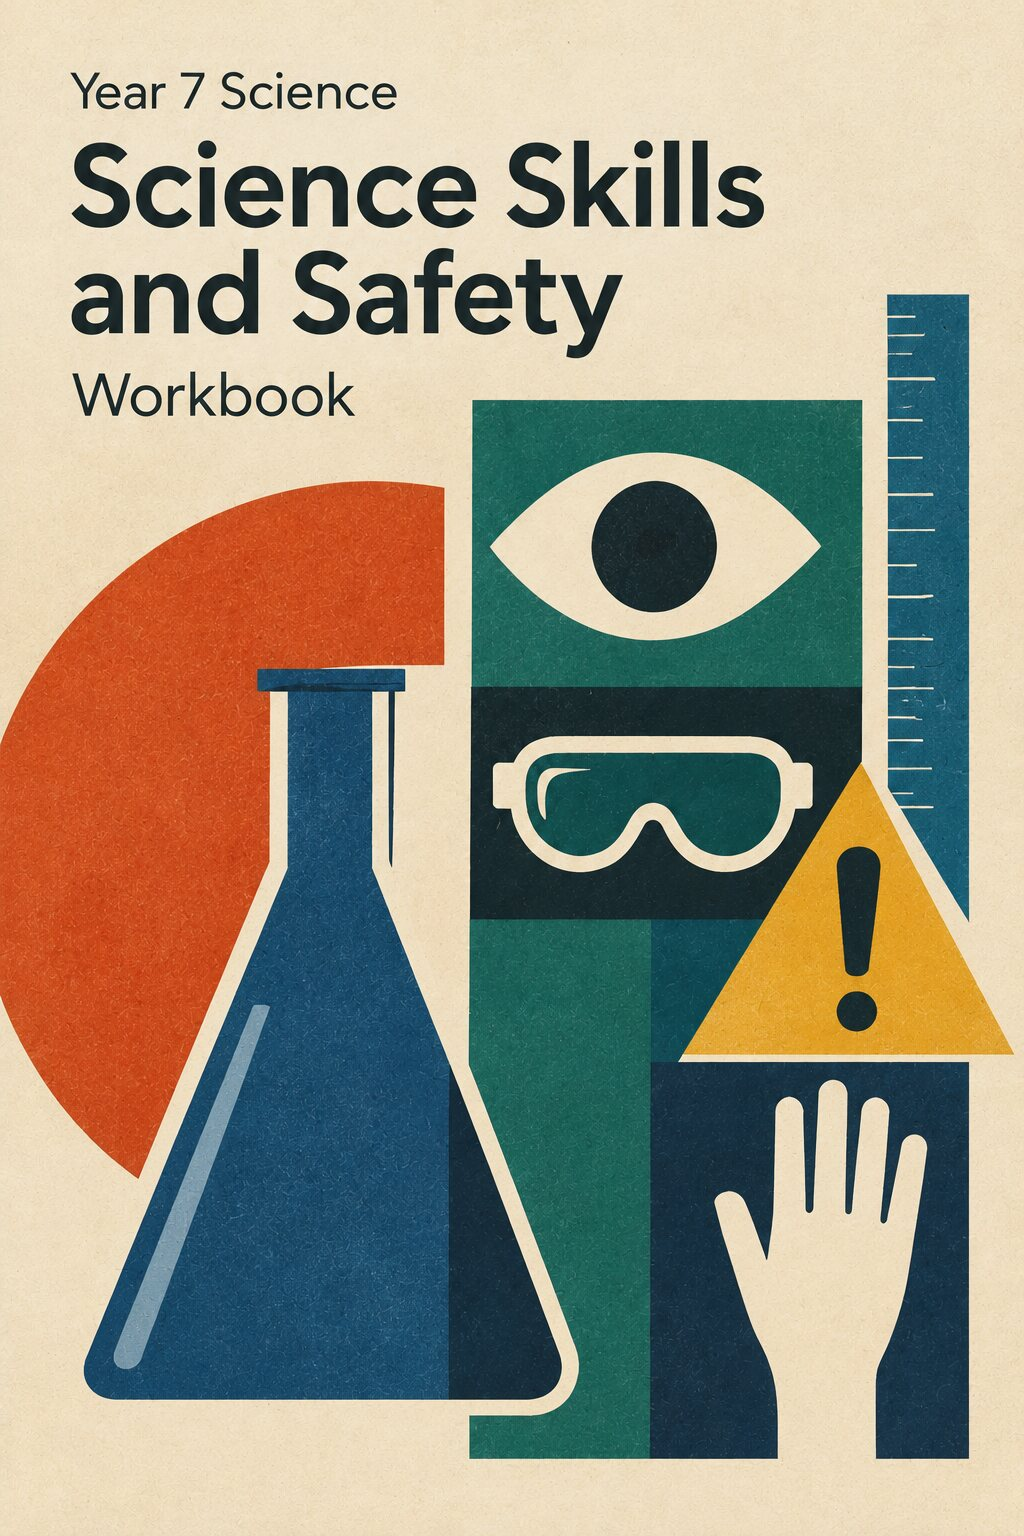
\includegraphics[width=\paperwidth]{../../covers/science-skills.jpg}};
  % Name box, top right, clear of the baked-in title ("Science Skills" ends ~140 mm in).
  \node[anchor=north east, fill=white, draw=Ink, line width=0.6pt, rounded corners=1.5mm,
        inner xsep=2.6mm, inner ysep=2.2mm, text width=40mm, font=\headingfont\small]
    at ([xshift=-6mm, yshift=-6mm]current page.north east)
    {\textbf{Name}\par\vspace{5mm}\hrule\vspace{2.6mm}\textbf{Class}\par\vspace{5mm}\hrule};
  % What this book is: the cover art says Workbook, so name the booklet here.
  \node[anchor=south east, fill=white, draw=Ink, line width=0.6pt, rounded corners=1.5mm,
        inner xsep=3.2mm, inner ysep=2.4mm, font=\headingfont\bfseries\large, align=right]
    at ([xshift=-6mm, yshift=8mm]current page.south east)
    {Experiment Booklet\\[-1pt]{\normalfont\headingfont\small Experiments 1--3}};
\end{tikzpicture}
\mbox{}
\clearpage

% ---- Inside cover ---------------------------------------------------------
\thispagestyle{plain}
{\headingfont\bfseries\fontsize{26}{30}\selectfont Science Skills and Safety}\par\vspace{1mm}
{\headingfont\Large Experiment Booklet \textbullet\ Year 7}\par\vspace{1mm}
{\small\itshape VC 2.0: VC2S8I01--I08 \textbullet\ VC2S8H01}\par\vspace{6mm}
\renewcommand{\arraystretch}{2.2}
\begin{tabular}{@{}l p{130mm}@{}}
\textbf{Name} & \hrulefill \\ \textbf{Class} & \hrulefill \\ \textbf{Teacher} & \hrulefill \\ \textbf{Lab group} & \hrulefill \\
\end{tabular}
\renewcommand{\arraystretch}{1}

\begin{countrybox}{Acknowledgement of Country}
This booklet was created on the unceded Country of the Wurundjeri Woi-wurrung people of the Kulin Nation. We acknowledge Elders past, present and emerging. Aboriginal and Torres Strait Islander peoples have observed, tested and passed on knowledge of Country for tens of thousands of years: science in the way this booklet teaches it, by careful observation, measurement and sharing what was found.
\end{countrybox}

\begin{infobox}{How this booklet works}
This booklet holds every experiment in the unit. Bring it to every practical lesson. Each experiment opens with its key vocabulary, learning intentions and skills focus, then runs \emph{Technique} $\rightarrow$ \emph{Plan and safety} $\rightarrow$ \emph{Method} $\rightarrow$ \emph{Results} $\rightarrow$ \emph{Analysis and evaluation} $\rightarrow$ \emph{Skill check}. Each kind of box has its own frame and mark:\par\smallskip
\renewcommand{\arraystretch}{1.35}
\begin{tabular}{@{}p{32mm}l@{}}
\textbf{Technique} \tagicon{\icokey} & How to do it properly (thin frame) \\
\textbf{I do} \tagicon{\icodots{1}} & Your teacher works an example through --- you follow (solid frame) \\
\textbf{We do} \tagicon{\icodots{2}} & You try one together, with help (dashed frame) \\
\textbf{You do} \tagicon{\icodots{3}} & On your own: check your understanding (heavy frame) \\
\textbf{Going further} \tagicon{\icoup} & Above level: Year 8 extension (double frame) \\
\textbf{Skills focus} \tagicon{\icoskill} & The science skills the experiment builds \\
\end{tabular}

\smallskip
Every skill comes from the faculty \textbf{Science Skills} list (the toolkit on page \pageref{sec:toolkit}). A skill always carries the same code, for example \sk{PC4} or \sk{PA1}, so you can follow it from this unit into every other unit this year.
\end{infobox}

\clearpage
{\headingfont\bfseries\LARGE Contents}\par\vspace{1mm}\noindent\rule{\linewidth}{0.6pt}\par\vspace{2mm}
\begin{ctab}
\renewcommand{\arraystretch}{1.5}
\begin{tabular}{|L{2.8cm}|L{10.2cm}|C{1.6cm}|}
  \hline\thead{Section} & \thead{Title} & \thead{Page} \\ \hline
  Skills & \hyperlink{toolkit}{The Science Skills toolkit} & \hyperlink{toolkit}{\pageref{sec:toolkit}} \\ \hline
  Skills & \hyperlink{tracker}{My skills tracker} & \hyperlink{tracker}{\pageref{sec:tracker}} \\ \hline
  Safety & \hyperlink{contract}{Lab safety contract (Lesson 5)} & \hyperlink{contract}{\pageref{sec:contract}} \\ \hline
  Experiment 1 & \hyperlink{exp.1}{Exploring the Lab (Lesson 2)} & \hyperlink{exp.1}{\pageref{sec:1}} \\ \hline
  Experiment 2 & \hyperlink{exp.2}{Measuring Mass and Volume (Lesson 3)} & \hyperlink{exp.2}{\pageref{sec:2}} \\ \hline
  Experiment 3 & \hyperlink{exp.3}{Measuring Temperature and Time (Lesson 6)} & \hyperlink{exp.3}{\pageref{sec:3}} \\ \hline
  Glossary & \hyperlink{glossary}{Key vocabulary, with the page each word first appears on} & \hyperlink{glossary}{\pageref{sec:glossary}} \\ \hline
\end{tabular}
\end{ctab}

% ══════════════════════════════════════════════════════════════════════════════
%  THE SCIENCE SKILLS TOOLKIT — faculty continuum, Years 7–8 column
% ══════════════════════════════════════════════════════════════════════════════
\clearpage
\hypertarget{toolkit}{}\pdfbookmark[1]{The Science Skills toolkit}{toolkitbm}
\markboth{The Science Skills toolkit}{}{\headingfont\bfseries\LARGE The Science Skills toolkit}\label{sec:toolkit}\par\vspace{1mm}\noindent\rule{\linewidth}{0.6pt}\par
These are the skills scientists use in every investigation. They come from the Science Inquiry strand of the Victorian Curriculum, grouped the way our faculty teaches them. Each experiment in this booklet tells you which skills it builds.

\newcommand{\tkhead}[2]{\multicolumn{3}{|l|}{\cellcolor{black!10}\rule{0pt}{4.6mm}\headingfont\bfseries #2} \\ \hline}
\newcommand{\tkrow}[1]{\skc{#1}\enspace{\small\bfseries\skname{#1}} & \skdesc{#1} & {\small\skcode{#1}} \\ \hline}
\renewcommand{\arraystretch}{1.35}
\begin{ctab}
\begin{longtable}{|W{5.0cm}|W{9.0cm}|Z{1.7cm}|}
  \hline\thead{Skill} & \thead{What it means} & \thead{Code} \\ \hline
  \endhead
  \tkhead{Teal}{Questioning and predicting}
  \tkrow{QP1}
  \tkrow{QP2}
  \tkhead{Blue}{Planning and conducting}
  \tkrow{PC1}
  \tkrow{PC2}
  \tkrow{PC3}
  \tkrow{PC4}
  \tkrow{PC5}
  \tkrow{PC6}
  \tkrow{PC7}
  \tkrow{PC8}
  \tkhead{GoldDark}{Processing, modelling and analysing}
  \tkrow{PA1}
  \tkrow{PA2}
  \tkrow{PA3}
  \tkrow{PA4}
  \tkrow{PA5}
  \tkrow{PA6}
  \tkrow{PA7}
  \tkrow{PA8}
  \tkhead{OrangeDark}{Evaluating}
  \tkrow{EV1}
  \tkrow{EV2}
  \tkrow{EV3}
  \tkrow{EV4}
  \tkrow{EV5}
  \tkhead{PurpleDark}{Communicating}
  \tkrow{CO1}
  \tkrow{CO2}
\end{longtable}
\end{ctab}
\renewcommand{\arraystretch}{1}

\begin{infobox}{Writing like a scientist \textbar\ CO1 \skname{CO1}}
Scientists write in the \textbf{third person}: say what was done, not who did it. Write \emph{``The water was heated for 10 minutes''}, not \emph{``I heated the water for 10 minutes''}. Keep sentences short, spell scientific words correctly, and always give a unit with a measurement.
\end{infobox}

% ══════════════════════════════════════════════════════════════════════════════
%  SKILLS TRACKER
% ══════════════════════════════════════════════════════════════════════════════
\clearpage
\hypertarget{tracker}{}\pdfbookmark[1]{My skills tracker}{trackerbm}
\markboth{My skills tracker}{}{\headingfont\bfseries\LARGE My skills tracker}\label{sec:tracker}\par\vspace{1mm}\noindent\rule{\linewidth}{0.6pt}\par
A dot \textbullet{} shows the experiments that build each skill. After each experiment, write how confident you are with each of its skills in its column: \textbf{1}~not yet, \textbf{2}~nearly, \textbf{3}~got it.

\newcommand{\dotc}{{\Large\textbullet}}
\newcommand{\trow}[4]{\rule[-0.36cm]{0pt}{0.92cm}\skc{#1}\enspace{\small\skname{#1}} & #2 & #3 & #4 & \\ \hline}
\begin{ctab}
\begin{tabular}{|W{5.6cm}|Z{1.8cm}|Z{1.8cm}|Z{1.8cm}|Z{2.3cm}|}
  \hline\thead{Skill} & \thead{Exp 1} & \thead{Exp 2} & \thead{Exp 3} & \thead{End of unit} \\ \hline
  \trow{QP1}{}{}{\dotc}
  \trow{PC1}{\dotc}{}{}
  \trow{PC2}{}{}{\dotc}
  \trow{PC3}{\dotc}{}{\dotc}
  \trow{PC4}{}{\dotc}{\dotc}
  \trow{PC6}{}{\dotc}{\dotc}
  \trow{PC7}{\dotc}{\dotc}{}
  \trow{PC8}{}{}{\dotc}
  \trow{PA1}{}{\dotc}{\dotc}
  \trow{PA3}{}{\dotc}{\dotc}
  \trow{PA5}{}{}{\dotc}
  \trow{PA7}{}{\dotc}{\dotc}
  \trow{EV1}{}{}{\dotc}
  \trow{EV2}{}{}{\dotc}
  \trow{EV3}{}{\dotc}{\dotc}
  \trow{CO1}{}{}{\dotc}
  \trow{CO2}{\dotc}{}{}
\end{tabular}
\end{ctab}
{\small\color{DarkGrey} Skills not in this unit (QP2, PC5, PA2, PA4, PA6, PA8, EV4, EV5) are built in the experiment booklets for later units. Graphing \sk{PA2} starts in The Particle Model, using your data from Experiment 3.}

% ══════════════════════════════════════════════════════════════════════════════
%  LAB SAFETY CONTRACT (Lesson 5)
% ══════════════════════════════════════════════════════════════════════════════
\clearpage
\hypertarget{contract}{}\pdfbookmark[1]{Lab safety contract}{contractbm}
\markboth{Lab safety contract}{}{\headingfont\bfseries\LARGE Lab safety contract}\label{sec:contract}\par\vspace{1mm}\noindent\rule{\linewidth}{0.6pt}\par
You sign this contract in Lesson 5, after the safety lesson and the safety quiz. You must pass the quiz and sign the contract before your next hands-on practical.\skr{PC3}

\begin{infobox}{In the laboratory I will \dots}
\begin{enumerate}[leftmargin=1.6em, itemsep=3pt]
  \item Enter the lab only when a teacher is present, and follow every instruction straight away.
  \item Wear safety glasses whenever chemicals, glassware or heat are being used.
  \item Tie back long hair, tuck in loose clothing and wear closed shoes.
  \item Keep bags under the bench and walkways clear.
  \item Never eat, drink or taste anything in the lab.
  \item Read the whole method before starting, and only do the experiment that has been approved.
  \item Smell a substance only by wafting it towards my nose, never by sniffing it directly.
  \item Point a heated test tube away from myself and other people.
  \item Report every spill, breakage, cut or burn to the teacher at once, however small.
  \item Put broken glass only in the broken-glass bin, never in the normal bin.
  \item Turn off the gas at the tap whenever a Bunsen burner is not being used.
  \item Clean my bench, wash my hands and return all equipment before I leave.
\end{enumerate}
\end{infobox}

\begin{scaffold}{If something goes wrong}
\textbf{Chemical in the eye:} use the eyewash station for at least 10 minutes. \quad
\textbf{Burn:} run cold water over it for 20 minutes. \quad
\textbf{Clothing on fire:} stop, drop and roll, or use the fire blanket. \quad
\textbf{Always:} tell the teacher straight away.
\end{scaffold}

\vspace{6pt}
I have read and understood the safety rules. I agree to follow them in every practical lesson. I understand that if I do not follow them I may be removed from practical work.

\vspace{12pt}
\begin{tabular}{@{}p{4.2cm}p{7cm}p{1.6cm}p{2.8cm}@{}}
  \textbf{Student signature:} & \underline{\hspace{6.6cm}} & \textbf{Date:} & \underline{\hspace{2.6cm}} \\[16pt]
  \textbf{Parent/guardian:}  & \underline{\hspace{6.6cm}} & \textbf{Date:} & \underline{\hspace{2.6cm}} \\[16pt]
  \textbf{Teacher:}          & \underline{\hspace{6.6cm}} & \textbf{Quiz:} & \underline{\hspace{2.6cm}} \\
\end{tabular}
% ══════════════════════════════════════════════════════════════════════════════
%  EXPERIMENT 1 — EXPLORING THE LAB                                    (Lesson 2)
% ══════════════════════════════════════════════════════════════════════════════
\experimentdiv{Exploring the Lab}{Naming lab equipment \textbullet{} Drawing scientific diagrams \textbullet{} Finding the safety equipment}{2}\label{sec:1}
\lessoncodes{VC2S8I02 \textbullet{} VC2S8I03 \textbullet{} VC2S8I08}

\vocabhead
\begin{ctab}
\begin{tabular}{|SW{4.2cm}|W{11.6cm}|}
  \hline\hd & \thead{Word} & \thead{Definition (copy from the slide)} \\ \hline
  & \scaf{\textbf{Hazard}\label{voc:hazard}} & \scaf{Anything that could cause harm, such as a flame, hot water or broken glass.} \\ \hline
  & \textbf{Risk}\label{voc:risk} & \\ \hline
  & \textbf{Control}\label{voc:control} & \\ \hline
  & \textbf{Equipment}\label{voc:equipment} & \\ \hline
  & \textbf{Scientific diagram}\label{voc:scientific-diagram} & \\ \hline
\end{tabular}
\end{ctab}

\begin{lipanel}
\inquiryli{Select the right equipment for a task and draw it as a scientific diagram.}
\understandli{Identify hazards in the lab and the equipment that controls them.}
\sctitle
\begin{itemize}[leftmargin=1.4em, itemsep=0pt, topsep=1pt]
  \item I can name ten pieces of lab equipment and say what each one is used for.
  \item I can draw three pieces of equipment as scientific diagrams.
  \item I can point to the safety equipment in our lab and name the hazard each one controls.
\end{itemize}
\end{lipanel}

\begin{skillsfocus}
\focus{PC7}{Name ten pieces of equipment and choose the right one for a job.}
\focus{PC3}{Find the safety equipment and match each piece to the hazard it controls.}
\focus{CO2}{Show equipment as scientific diagrams: the way scientists draw an experiment.}
\focus{PC1}{Work through the stations in order and follow each instruction card.}
\end{skillsfocus}

% ─── TECHNIQUE ────────────────────────────────────────────────────────────────
\exppart{Technique spotlight}{Blue}

\begin{technique}{Drawing a scientific diagram}{CO2}
A scientific diagram shows equipment as a simple, flat outline, so anyone can see quickly how an experiment is set up. Follow these six rules every time.
\begin{enumerate}[leftmargin=1.6em, itemsep=1pt, topsep=3pt]
  \item Use a \textbf{sharp pencil}, never a pen.
  \item Use a \textbf{ruler} for every straight line.
  \item Draw the equipment \textbf{side-on and flat (2D)}: no 3D shapes, no shading, no colouring in.
  \item Leave the top of an open container \textbf{open}.
  \item Label each part with a \textbf{ruled line} that touches the part. Write labels at the side. Label lines never cross.
  \item Give the diagram a \textbf{title} that says what it shows.
\end{enumerate}
\end{technique}

\begin{center}
\begin{tikzpicture}[scale=0.65]
  % a realistic sketch: 3D rim, shading
  \begin{scope}
    \shade[left color=LightGrey, right color=MidGrey!80] (0,0) arc[start angle=180,end angle=360,x radius=0.9,y radius=0.22] -- (1.8,2.5) arc[start angle=0,end angle=-180,x radius=0.9,y radius=0.22] -- cycle;
    \draw[Ink, line width=0.8pt] (0.9,2.5) ellipse (0.9 and 0.22);
    \draw[Ink, line width=0.8pt] (0,2.5) -- (0,0) arc[start angle=180,end angle=360,x radius=0.9,y radius=0.22] -- (1.8,2.5);
    \fill[Sky!45] (0.02,1.2) arc[start angle=180,end angle=360,x radius=0.88,y radius=0.2] -- (1.78,0.02) arc[start angle=0,end angle=-180,x radius=0.88,y radius=0.2] -- cycle;
    \node[font=\footnotesize\bfseries, text=OrangeDark] at (0.9,-0.75) {\ding{55}\ A sketch, not a scientific diagram};
  \end{scope}
  % the scientific diagram
  \begin{scope}[xshift=7cm]
    \draw[Sky!60, line width=0.6pt] (0,1.2) -- (1.8,1.2);
    \eqBeaker
    \eqlab{(1.8,2.2)}{(2.6,2.2)}{beaker}
    \eqlab{(1.2,1.2)}{(2.6,1.2)}{water}
    \node[font=\footnotesize\bfseries, text=TealGreen] at (1.25,-0.75) {\ding{51}\ A scientific diagram};
  \end{scope}
\end{tikzpicture}
\expfigcap{The same beaker of water drawn two ways.}
\end{center}

\begin{workedex}{A conical flask of water}
\begin{minipage}[c]{0.5\linewidth}
\textbf{Task:} Draw a conical flask half full of water as a scientific diagram.

\smallskip
\textbf{How:} The flask is drawn side-on in ruled pencil lines. The water is a single ruled line across the flask, at its level. The top of the flask is left open. Each label sits at the side on a ruled line that touches the part.
\end{minipage}\hfill
\begin{minipage}[c]{0.44\linewidth}\centering
\begin{tikzpicture}
  \draw[Sky!60, line width=0.6pt] (0.32,1.0) -- (1.58,1.0);
  \eqFlask
  \eqlab{(1.25,2.5)}{(2.4,2.5)}{conical flask}
  \eqlab{(1.2,1.0)}{(2.4,1.0)}{water}
  \node[font=\footnotesize\bfseries] at (1.0,-0.45) {A conical flask of water};
\end{tikzpicture}
\end{minipage}
\end{workedex}

\begin{wedo}{A filter funnel in a conical flask}
Draw a filter funnel sitting in the neck of a conical flask as a scientific diagram. Label both pieces of equipment and give your diagram a title.
\drawbox{4.5cm}{}
\end{wedo}

% ─── PLAN AND SAFETY / METHOD ────────────────────────────────────────────────
\exppart{Plan, safety and method}{Teal}

\textbf{Aim:} To identify common laboratory equipment and the safety equipment in our lab, and to draw equipment as scientific diagrams.\skr{PC1}

\begin{infobox}{Safety}
Do not light, heat or plug in anything during this lesson. Carry glassware with two hands and put it down away from the edge of the bench. Report any chipped or broken glass to your teacher: do not pick it up.
\end{infobox}

\subsubsection*{Method --- Part 1: Equipment stations}
\begin{enumerate}[itemsep=2pt]
  \item Your teacher has set out ten numbered stations around the room, each with one piece of equipment and an instruction card.
  \item Start at the station your teacher gives you. Move to the next number when your teacher says to.
  \item At each station, find the matching drawing in the table in your results, then write the equipment's name and what it is used for.
  \item Handle each piece carefully and leave it exactly as you found it.
\end{enumerate}

\subsubsection*{Method --- Part 2: Safety equipment hunt}
\begin{enumerate}[itemsep=2pt]
  \item With your group, walk around the lab and find each piece of safety equipment listed in your results. Do not touch the safety shower, eyewash or fire equipment.
  \item Record where each one is, and the hazard it controls.
  \item Back at your bench, draw a map of the lab and mark where each piece of safety equipment is.
\end{enumerate}

\begin{scaffold}{Word bank --- equipment}
beaker \textbullet{} conical flask \textbullet{} test tube \textbullet{} measuring cylinder \textbullet{} filter funnel \textbullet{} evaporating basin \textbullet{} tripod and gauze mat \textbullet{} Bunsen burner \textbullet{} thermometer \textbullet{} retort stand and clamp
\end{scaffold}

% ─── RESULTS ─────────────────────────────────────────────────────────────────
\exppart{Results}{Amber}

\subsubsection*{Results --- Part 1: Equipment stations \hfill \sk{PC7}}
\newcommand{\eqcell}[2][0.5]{\raisebox{-0.5\height}{\eqpic[#1]{#2}}}
\begin{ctab}
\begin{tabular}{|SZ{1.0cm}|Z{2.6cm}|W{4.0cm}|W{7.6cm}|}
  \hline\hd & \thead{No.} & \thead{Diagram} & \thead{Name} & \thead{What it is used for} \\ \hline
  & \scaf{e.g.} & \eqcell{\eqBeaker} & \scaf{Beaker} & \scaf{Holding, mixing and heating liquids. Its markings only give a rough volume.} \\ \hline
  & 1 & \eqcell{\eqFlask} & & \\ \hline
  & 2 & \eqcell{\eqTestTube} & & \\ \hline
  & 3 & \eqcell[0.42]{\eqCylinder} & & \\ \hline
  & 4 & \eqcell{\eqFunnel} & & \\ \hline
  & 5 & \eqcell{\eqBasin} & & \\ \hline
  & 6 & \eqcell{\eqTripod} & & \\ \hline
  & 7 & \eqcell{\eqBunsen} & & \\ \hline
  & 8 & \eqcell[0.42]{\eqThermometer} & & \\ \hline
  & 9 & \eqcell[0.42]{\eqStand} & & \\ \hline
\end{tabular}
\end{ctab}

\needspace{12\baselineskip}
\task Choose three pieces of equipment from the stations. Draw each one as a scientific diagram, following all six rules. Label and title each diagram.\skr{CO2}

\noindent
\begin{minipage}[t]{0.32\linewidth}\drawbox{6cm}{}\nameline{Title:}\end{minipage}\hfill
\begin{minipage}[t]{0.32\linewidth}\drawbox{6cm}{}\nameline{Title:}\end{minipage}\hfill
\begin{minipage}[t]{0.32\linewidth}\drawbox{6cm}{}\nameline{Title:}\end{minipage}

\clearpage
\subsubsection*{Results --- Part 2: Safety equipment hunt \hfill \sk{PC3}}
\begin{ctab}
\begin{tabular}{|SW{4.0cm}|W{4.6cm}|W{6.6cm}|}
  \hline\hd & \thead{Safety equipment} & \thead{Where it is in our lab} & \thead{The hazard it controls} \\ \hline
  & \scaf{Fire blanket} & \scaf{On the wall beside the front door} & \scaf{Fire: it smothers a small fire, or clothing that has caught fire} \\ \hline
  & Fire extinguisher & & \\ \hline
  & Eyewash station & & \\ \hline
  & Safety shower & & \\ \hline
  & First-aid kit & & \\ \hline
  & Emergency gas shut-off & & \\ \hline
  & Safety glasses & & \\ \hline
  & Broken-glass bin & & \\ \hline
  & Spill kit & & \\ \hline
\end{tabular}
\end{ctab}

\needspace{12\baselineskip}
\task Draw a bird's-eye map of the lab: the walls, doors and benches. Mark each piece of safety equipment with its first letter, and add a key.
\drawbox{8cm}{}

% ─── ANALYSIS ────────────────────────────────────────────────────────────────
\exppart{Analysis and evaluation}{Coral}

\task Explain the difference between a \emph{hazard} and a \emph{risk}. Use a lit Bunsen burner as your example.
\answerbox{5cm}

\needspace{12\baselineskip}
\task Complete the table: for each hazard, name the safety equipment you would use, or the rule that prevents it.\skr{PC3}
\begin{ctab}
\begin{tabular}{|SW{6.6cm}|W{8.6cm}|}
  \hline\hd & \thead{Hazard} & \thead{Safety equipment or rule that controls it} \\ \hline
  & \scaf{Long hair near a Bunsen flame} & \scaf{Tie long hair back before lighting a Bunsen burner.} \\ \hline
  & A chemical splashes into someone's eye & \\ \hline
  & A beaker is knocked off the bench and breaks & \\ \hline
  & Water is spilt on the floor & \\ \hline
  & A student's sleeve catches fire & \\ \hline
\end{tabular}
\end{ctab}

\needspace{10\baselineskip}
\task Scientists draw equipment as flat outlines instead of realistic pictures. Give two reasons why.\skr{CO2}
\answerbox{5cm}

\needspace{12\baselineskip}
\task Name the best piece of equipment for each job. Choose from: beaker, measuring cylinder, filter funnel, test-tube holder, thermometer, evaporating basin.\skr{PC7}
\pt{a}Measuring exactly 35\,mL of water.
\answerbox{1cm}
\pt{b}Heating 100\,mL of water.
\answerbox{1cm}
\pt{c}Separating sand from water.
\answerbox{1cm}
\pt{d}Holding a test tube above a flame.
\answerbox{1cm}
\pt{e}Measuring how hot some water is.
\answerbox{1cm}

\begin{yr8box}
\begin{keepext}
\exttask A measuring cylinder is never heated over a Bunsen burner, but a beaker often is. Suggest why, thinking about what each piece of equipment is designed to do well.
\answerbox{5cm}
\end{keepext}
\end{yr8box}

% ─── SKILL CHECK ─────────────────────────────────────────────────────────────
\exppart{Skill check}{NavyBlue}

\begin{skillcheck}
\scrow{PC7}{I can name ten pieces of lab equipment and say what each one is used for.}
\scrow{CO2}{I can draw equipment as a scientific diagram: pencil, ruler, 2D outline, ruled labels and a title.}
\scrow{PC3}{I can point to each piece of safety equipment in our lab and name the hazard it controls.}
\scrow{PC1}{I followed the station instructions in order and left each station as I found it.}
\end{skillcheck}

\task Which piece of equipment are you least sure about? Write what you will do to learn it before the next practical.
\answerbox{5cm}
% ══════════════════════════════════════════════════════════════════════════════
%  EXPERIMENT 2 — MEASURING MASS AND VOLUME                            (Lesson 3)
% ══════════════════════════════════════════════════════════════════════════════
\experimentdiv{Measuring Mass and Volume}{Using an electronic balance \textbullet{} Reading a measuring cylinder \textbullet{} Precision}{3}\label{sec:2}
\lessoncodes{VC2S8I02 \textbullet{} VC2S8I03 \textbullet{} VC2S8I04 \textbullet{} VC2S8I05 \textbullet{} VC2S8I06}

\vocabhead
\begin{ctab}
\begin{tabular}{|SW{4.2cm}|W{11.6cm}|}
  \hline\hd & \thead{Word} & \thead{Definition (copy from the slide)} \\ \hline
  & \scaf{\textbf{Mass}\label{voc:mass}} & \scaf{The amount of matter in an object, measured in grams (g) or kilograms (kg).} \\ \hline
  & \textbf{Volume}\label{voc:volume} & \\ \hline
  & \textbf{Meniscus}\label{voc:meniscus} & \\ \hline
  & \textbf{Tare}\label{voc:tare} & \\ \hline
  & \textbf{Precision}\label{voc:precision} & \\ \hline
\end{tabular}
\end{ctab}

\begin{lipanel}
\inquiryli{Use equipment to collect precise measurements and record them in a table with units.}
\understandli{Explain the difference between mass and volume.}
\sctitle
\begin{itemize}[leftmargin=1.4em, itemsep=0pt, topsep=1pt]
  \item I can tare an electronic balance and record a mass with its unit.
  \item I can read a measuring cylinder at eye level, from the bottom of the meniscus.
  \item I can record measurements in a table with the units in the column headings.
  \item I can explain the difference between mass and volume.
\end{itemize}
\end{lipanel}

\begin{skillsfocus}
\focus{PC4}{Read each scale to its smallest division, and choose the cylinder with the finest scale.}
\focus{PC6}{Measure each object three times and record every reading with its unit.}
\focus{PC7}{Use an electronic balance and a measuring cylinder correctly.}
\focus{PA1}{Record your data in tables, with units in the headings.}
\focus{PA3}{Calculate an average and a difference from your data.}
\end{skillsfocus}

% ─── TECHNIQUE ────────────────────────────────────────────────────────────────
\exppart{Technique spotlight}{Blue}

\begin{technique}{Using an electronic balance}{PC7}
\begin{minipage}[c]{0.6\linewidth}
\begin{enumerate}[leftmargin=1.6em, itemsep=1pt, topsep=0pt]
  \item Put the balance on a flat, steady bench, away from water.
  \item Press \textbf{TARE} with nothing on the pan, so it reads 0.00\,g.
  \item Place the object gently in the middle of the pan.
  \item Wait until the number stops changing.
  \item Record \textbf{every} digit shown, and the unit.
\end{enumerate}
\end{minipage}\hfill
\begin{minipage}[c]{0.36\linewidth}\centering
\balancefig{24.68\,g}\\[2pt]
{\footnotesize Record this as \textbf{24.68\,g}, not 24.7\,g.}
\end{minipage}

\medskip
\textbf{Taring with a container.} To find the mass of a liquid, put the empty beaker on the pan and press \textbf{TARE}. The balance now reads 0.00\,g, so when you pour in the liquid it shows the mass of the liquid alone.
\end{technique}

\begin{workedex}{The mass of some water without taring}
A beaker has a mass of 52.30\,g. With water in it, the balance reads 87.65\,g. Find the mass of the water.

\smallskip
\textbf{Working:} mass of water $=$ (beaker $+$ water) $-$ beaker $= 87.65 - 52.30 = 35.35$\,g.
\end{workedex}

\begin{wedo}{The mass of some water without taring}
A beaker has a mass of 48.20\,g. With water in it, the balance reads 83.65\,g. Find the mass of the water.
\workbox{3cm}
\end{wedo}

\begin{technique}{Reading a measuring cylinder}{PC4}
\begin{minipage}[c]{0.64\linewidth}
\begin{enumerate}[leftmargin=1.6em, itemsep=1pt, topsep=0pt]
  \item Stand the cylinder on a flat bench. Do not hold it up.
  \item \textbf{Work out the scale.} Take two labelled marks, find the difference between them, and divide by the number of spaces between them. That is the value of one small division.
  \item Bend down so your eye is \textbf{level} with the top of the water. Looking from above or below gives the wrong reading (\emph{parallax error}).
  \item Water curves down in the middle. This curve is the \textbf{meniscus}. Read the scale at the \textbf{bottom} of the meniscus.
  \item Record the reading and the unit, mL.
\end{enumerate}
\end{minipage}\hfill
\begin{minipage}[c]{0.32\linewidth}\centering
\begin{tikzpicture}
  \fill[Sky!22] (0,0) -- (0,1.36) .. controls (0.6,1.0) and (1.6,1.0) .. (2.2,1.36) -- (2.2,0) -- cycle;
  \draw[Ink, line width=0.9pt] (0,1.36) .. controls (0.6,1.0) and (1.6,1.0) .. (2.2,1.36);
  \draw[eq] (0,0) -- (0,2.2) (2.2,0) -- (2.2,2.2);
  \draw[OrangeDark, line width=0.8pt, dashed] (-0.3,1.09) -- (2.5,1.09);
  \node[font=\scriptsize, align=center, anchor=north] at (1.1,-0.05) {read the scale\\at the bottom\\of the meniscus};
  \node[font=\scriptsize] at (3.05,1.09) {eye};
  \fill[Ink] (2.75,1.09) circle (1.2pt);
\end{tikzpicture}
\end{minipage}
\end{technique}

\begin{workedex}{Reading a measuring cylinder}
\begin{minipage}[c]{0.64\linewidth}
Read the volume of water in this measuring cylinder.

\smallskip
\textbf{Scale:} the labelled marks 30 and 40 are 10\,mL apart, with 10 spaces between them. One small division is $10 \div 10 = 1$\,mL.

\smallskip
\textbf{Reading:} the bottom of the meniscus is 4 small divisions above 30, so the volume is $30 + 4 \times 1 = $ \textbf{34\,mL}.
\end{minipage}\hfill
\begin{minipage}[c]{0.3\linewidth}\centering
\readcyl{20}{50}{10}{10}{34}
\end{minipage}
\end{workedex}

\begin{wedo}{Reading a measuring cylinder}
\begin{minipage}[c]{0.64\linewidth}
\pt{a}What is the value of one small division?
\workbox{2.2cm}
\pt{b}Read the volume of water.
\answerbox{1cm}
\end{minipage}\hfill
\begin{minipage}[c]{0.3\linewidth}\centering
\readcyl{0}{25}{5}{5}{17}
\end{minipage}
\end{wedo}

\begin{technique}{Choosing the most precise equipment}{PC4}
The smaller the value of one small division, the more \textbf{precise} the measurement. Choose the \textbf{smallest} measuring cylinder that holds the whole volume. A 10\,mL cylinder can be read to 0.2\,mL, but a 250\,mL cylinder only to 10\,mL.
\end{technique}

\begin{workedex}{Choosing a measuring cylinder}
You need 8\,mL of water. You have a 10\,mL, a 50\,mL and a 100\,mL measuring cylinder.

\smallskip
\textbf{Choice:} the \textbf{10\,mL} cylinder. It holds 8\,mL and has the smallest divisions (0.2\,mL), so the reading is the most precise. In the 100\,mL cylinder, 8\,mL barely covers the base.
\end{workedex}

\begin{wedo}{Choosing a measuring cylinder}
You need 45\,mL of water. You have a 10\,mL, a 50\,mL and a 250\,mL measuring cylinder. Choose one and explain your choice.
\answerbox{5cm}
\end{wedo}

\begin{youdobox}[Reading measuring cylinders]
\task Read each measuring cylinder. Give the value of one small division and the volume, with units.\skr{PC4}

\begin{center}
\begin{tabular}{ccc}
  \readcyl{4}{9}{1}{5}{6.4} & \hspace{1.2cm}\readcyl{50}{100}{10}{5}{76} & \hspace{1.2cm}\readcyl{100}{250}{50}{5}{180} \\[4pt]
  \textbf{(a)} & \hspace{1.2cm}\textbf{(b)} & \hspace{1.2cm}\textbf{(c)} \\
\end{tabular}
\end{center}
\begin{ctab}
\begin{tabular}{|SZ{1.6cm}|Z{6.2cm}|Z{6.2cm}|}
  \hline\hd & \thead{Cylinder} & \thead{Value of one small division (mL)} & \thead{Volume (mL)} \\ \hline
  & \scaf{e.g.} & \scaf{1} & \scaf{34} \\ \hline
  & (a) & & \\ \hline
  & (b) & & \\ \hline
  & (c) & & \\ \hline
\end{tabular}
\end{ctab}
\end{youdobox}

% ─── PLAN AND SAFETY / METHOD ────────────────────────────────────────────────
\exppart{Plan, safety and method}{Teal}

\textbf{Aim:} To measure mass and volume precisely, and to find out which equipment measures volume most precisely.\skr{PC1}

\subsubsection*{Equipment}
\begin{multicols}{2}
\begin{itemize}[leftmargin=1.2em, itemsep=0pt, topsep=0pt]
  \item electronic balance (reads to 0.01\,g)
  \item marble, rubber stopper, 10 paper clips
  \item 100\,mL beaker
  \item four measuring cylinders, filled by your teacher (B1--B4)
  \item 250\,mL beaker with markings
  \item 50\,mL and 100\,mL measuring cylinders
  \item wash bottle of water, paper towel
\end{itemize}
\end{multicols}

\begin{infobox}{Safety}
Keep water well away from the balance and its power cord, and wipe up any spill straight away. Carry measuring cylinders by the body, not the rim; they tip over easily, so stand them away from the bench edge. Report broken glass to your teacher.
\end{infobox}

\subsubsection*{Station A --- Mass \hfill \sk{PC6}}
\begin{enumerate}[itemsep=2pt]
  \item Tare the balance so it reads 0.00\,g.
  \item Place the first object in the middle of the pan. Record its mass in Table A.
  \item Take the object off, check the balance reads 0.00\,g again, and repeat until a different person in your group has measured it each time (three trials).
  \item Repeat for each object, then calculate each average.
\end{enumerate}

\subsubsection*{Station B --- Volume}
\begin{enumerate}[itemsep=2pt]
  \item For each cylinder B1--B4, work out the value of one small division.
  \item Read the volume at eye level, from the bottom of the meniscus. Record it in Table B. Do not pick the cylinder up.
\end{enumerate}

\subsubsection*{Station C --- The precision challenge}
\begin{enumerate}[itemsep=2pt]
  \item Put the empty 100\,mL beaker on the balance and press \textbf{TARE}.
  \item Measure 35\,mL of water using the markings on the 250\,mL beaker. Pour it into the beaker on the balance and record its mass in Table C.
  \item Empty and dry the beaker, tare again, and repeat with the 100\,mL measuring cylinder, then the 50\,mL measuring cylinder.
  \item One millilitre of water has a mass of 1\,g, so a perfect 35\,mL would read 35.00\,g. Calculate how far each result is from 35.00\,g.
\end{enumerate}

% ─── RESULTS ─────────────────────────────────────────────────────────────────
\exppart{Results}{Amber}

\subsubsection*{Table A --- The mass of four objects \hfill \sk{PA1}}
\begin{ctab}
\begin{tabular}{|SW{3.6cm}|Z{2.6cm}|Z{2.6cm}|Z{2.6cm}|Z{3.2cm}|}
  \hline\hd & \thead{Object} & \thead{Trial 1 (g)} & \thead{Trial 2 (g)} & \thead{Trial 3 (g)} & \thead{Average (g)} \\ \hline
  & \scaf{e.g. eraser} & \scaf{21.36} & \scaf{21.35} & \scaf{21.36} & \scaf{21.36} \\ \hline
  & Marble & & & & \\ \hline
  & Rubber stopper & & & & \\ \hline
  & 10 paper clips & & & & \\ \hline
  & 100\,mL beaker & & & & \\ \hline
\end{tabular}
\end{ctab}

\begin{scaffold}{Calculating an average \textbar\ PA3 \skname{PA3}}
Add the three trials and divide by 3. Round to the same number of decimal places as the readings.\quad
e.g.\ $(21.36 + 21.35 + 21.36) \div 3 = 64.07 \div 3 = 21.356\ldots \approx 21.36$\,g
\end{scaffold}

\subsubsection*{Table B --- Reading measuring cylinders}
\begin{ctab}
\begin{tabular}{|SZ{2.4cm}|Z{3.6cm}|Z{4.6cm}|Z{4.4cm}|}
  \hline\hd & \thead{Cylinder} & \thead{Size of cylinder (mL)} & \thead{Value of one small division (mL)} & \thead{Volume (mL)} \\ \hline
  & \scaf{e.g.} & \scaf{25} & \scaf{0.5} & \scaf{18.5} \\ \hline
  & B1 & & & \\ \hline
  & B2 & & & \\ \hline
  & B3 & & & \\ \hline
  & B4 & & & \\ \hline
\end{tabular}
\end{ctab}

\subsubsection*{Table C --- Measuring 35\,mL three ways}
\begin{ctab}
\begin{tabular}{|SW{5.6cm}|Z{4.4cm}|Z{5.4cm}|}
  \hline\hd & \thead{Equipment used to measure 35\,mL} & \thead{Mass of water (g)} & \thead{Difference from 35.00\,g (g)} \\ \hline
  & \scaf{e.g. markings on a conical flask} & \scaf{37.80} & \scaf{$37.80 - 35.00 = 2.80$} \\ \hline
  & Markings on the 250\,mL beaker & & \\ \hline
  & 100\,mL measuring cylinder & & \\ \hline
  & 50\,mL measuring cylinder & & \\ \hline
\end{tabular}
\end{ctab}

% ─── ANALYSIS ────────────────────────────────────────────────────────────────
\exppart{Analysis and evaluation}{Coral}

\task Explain the difference between mass and volume. Give the unit you used for each.
\answerbox{5cm}

\needspace{10\baselineskip}
\task Look at your three trials for each object in Table A. How close together were they, and what does this tell you about the precision of the balance?\skr{PC4}
\answerbox{5cm}

\needspace{14\baselineskip}
\task A group recorded these masses for a marble: 5.62\,g, 5.61\,g and 5.16\,g.\skr{PA7}
\pt{a}Which reading is the anomaly?
\answerbox{1cm}
\pt{b}Suggest what might have caused it.
\answerbox{5cm}
\pt{c}What should the group do about it before they calculate an average?
\answerbox{5cm}

\needspace{10\baselineskip}
\task Which equipment measured 35\,mL of water most precisely in Table C? Quote your results as evidence.\skr{PC4}
\answerbox{5cm}

\needspace{10\baselineskip}
\task Why is the unit written once in each column heading, instead of after every number in the table?\skr{PA1}
\answerbox{5cm}

\needspace{14\baselineskip}
\task Readings from a measuring cylinder can be wrong.\skr{EV3}
\pt{a}Describe one mistake that gives a wrong reading, and how to avoid it.
\answerbox{5cm}
\pt{b}Describe a different mistake, and how to avoid it.
\answerbox{5cm}

\needspace{8\baselineskip}
\task A beaker has a mass of 64.15\,g. With water in it, it has a mass of 112.40\,g. Calculate the mass of the water.\skr{PA3}
\workbox{3.5cm}

\begin{yr8box}
\begin{keepext}
\exttask A kitchen scale reads to the nearest 1\,g. The lab balance reads to 0.01\,g. A 10-cent coin has a mass of about 5.65\,g. Which would you use to measure the coin's mass, and why?
\answerbox{5cm}
\end{keepext}
\begin{keepext}
\exttask A student measures 7\,mL of water in a 100\,mL measuring cylinder whose small divisions are 1\,mL. Explain why this is a poor choice, and how much better a 10\,mL cylinder with 0.2\,mL divisions would be.
\answerbox{5cm}
\end{keepext}
\end{yr8box}

% ─── SKILL CHECK ─────────────────────────────────────────────────────────────
\exppart{Skill check}{NavyBlue}

\begin{skillcheck}
\scrow{PC7}{I can tare an electronic balance and record a mass with every digit and its unit.}
\scrow{PC4}{I can read a measuring cylinder at eye level from the bottom of the meniscus, and choose the most precise cylinder.}
\scrow{PC6}{I measured each object three times and recorded every reading straight away.}
\scrow{PA1}{I can record data in a table with the units in the column headings.}
\scrow{PA3}{I can calculate an average and a difference.}
\scrow{PA7}{I can spot a reading that does not fit with the others.}
\scrow{EV3}{I can name a mistake that makes a reading wrong, and how to avoid it.}
\end{skillcheck}

\task Which skill on this page will you focus on in the next experiment? Explain what you will do differently.
\answerbox{5cm}
% ══════════════════════════════════════════════════════════════════════════════
%  EXPERIMENT 3 — MEASURING TEMPERATURE AND TIME                       (Lesson 6)
% ══════════════════════════════════════════════════════════════════════════════
\experimentdiv{Measuring Temperature and Time}{Using a Bunsen burner safely \textbullet{} Reading a thermometer \textbullet{} Recording at regular intervals}{6}\label{sec:3}
\lessoncodes{VC2S8I01--I06 \textbullet{} VC2S8I08}

\vocabhead
\begin{ctab}
\begin{tabular}{|SW{4.2cm}|W{11.6cm}|}
  \hline\hd & \thead{Word} & \thead{Definition (copy from the slide)} \\ \hline
  & \scaf{\textbf{Temperature}\label{voc:temperature}} & \scaf{How hot or cold something is, measured in degrees Celsius (\textdegree C).} \\ \hline
  & \textbf{Thermometer}\label{voc:thermometer} & \\ \hline
  & \textbf{Interval}\label{voc:interval} & \\ \hline
  & \textbf{Safety flame}\label{voc:safety-flame} & \\ \hline
  & \textbf{Heating flame}\label{voc:heating-flame} & \\ \hline
\end{tabular}
\end{ctab}

\begin{lipanel}
\inquiryli{Use equipment safely to record temperature at regular time intervals in a table.}
\understandli{Describe how the temperature of water changes as it is heated.}
\sctitle
\begin{itemize}[leftmargin=1.4em, itemsep=0pt, topsep=1pt]
  \item I can light a Bunsen burner safely and switch between the safety flame and the heating flame.
  \item I can read a thermometer at eye level to the nearest degree.
  \item I can record the temperature of heating water every minute in a table, and describe the pattern.
\end{itemize}
\end{lipanel}

\begin{skillsfocus}
\focus{QP1}{Write a prediction you can test, as \emph{If \dots\ then \dots\ because \dots}}
\focus{PC2}{Name the independent, dependent and controlled variables.}
\focus{PC3}{Complete a risk assessment before you light the Bunsen burner.}
\focus{PC4}{Read the thermometer at eye level, to the nearest degree.}
\focus{PC6}{Take a reading at every whole minute, with its unit.}
\focus{PA5}{Describe the pattern: how temperature changes with time.}
\focus{EV2}{Compare your boiling point with the accepted value, 100\,\textdegree C.}
\end{skillsfocus}

% ─── TECHNIQUE ────────────────────────────────────────────────────────────────
\exppart{Technique spotlight}{Blue}

\begin{technique}{Using a Bunsen burner}{PC3}
\begin{minipage}[c]{0.62\linewidth}
\textbf{Before you light it}
\begin{itemize}[leftmargin=1.2em, itemsep=0pt, topsep=1pt]
  \item Safety glasses on, hair tied back, sleeves tucked in, bag under the bench.
  \item Stand the burner on a heatproof mat, away from paper and the bench edge.
  \item Check the gas tube for cracks, and push it firmly onto the gas tap.
\end{itemize}
\smallskip
\textbf{Lighting it}
\begin{enumerate}[leftmargin=1.6em, itemsep=0pt, topsep=1pt]
  \item Turn the collar so the air hole is \textbf{closed}.
  \item Light the match or striker \textbf{first}, and hold it beside the top of the barrel.
  \item Turn the gas tap on. You get the yellow \textbf{safety flame}.
  \item To heat, open the air hole to get the blue \textbf{heating flame}.
  \item Whenever you are not heating, close the air hole to show the safety flame.
  \item When you finish, turn the gas tap off.
\end{enumerate}
\end{minipage}\hfill
\begin{minipage}[c]{0.34\linewidth}\centering
\bunsenflame{safety}\hspace{0.5cm}\bunsenflame{heating}\\[3pt]
{\footnotesize\textbf{Safety flame}\hspace{0.6cm}\textbf{Heating flame}}\\[2pt]
{\scriptsize air hole closed: yellow, wavy, easy to see\\[1pt] air hole open: blue, hot, hard to see}
\end{minipage}
\end{technique}

\begin{youdobox}[The parts of a Bunsen burner]
\task Name each labelled part of the Bunsen burner. Choose from: \emph{air hole, barrel, base, collar, gas tube.}\skr{PC7}

\noindent
\begin{minipage}[c]{0.36\linewidth}\centering
\begin{tikzpicture}[scale=1.25]
  \eqBunsen
  \draw[eqlab] (0.58,2.0) -- (-0.4,2.0) node[eqtext, anchor=east, font=\bfseries\small] {A};
  \draw[eqlab] (1.1,0.75) -- (1.9,0.95) node[eqtext, anchor=west, font=\bfseries\small] {B};
  \draw[eqlab] (0.8,0.52) -- (1.9,0.45) node[eqtext, anchor=west, font=\bfseries\small] {C};
  \draw[eqlab] (1.6,0.1) -- (1.9,-0.1) node[eqtext, anchor=west, font=\bfseries\small] {D};
  \draw[eqlab] (-0.4,0.11) -- (-0.6,-0.3) node[eqtext, anchor=north, font=\bfseries\small] {E};
\end{tikzpicture}
\end{minipage}\hfill
\begin{minipage}[c]{0.6\linewidth}
\begin{ctab}
\begin{tabular}{|SZ{1.2cm}|W{6.6cm}|}
  \hline\hd & \thead{Part} & \thead{Name} \\ \hline
  & \scaf{A} & \scaf{Barrel} \\ \hline
  & B & \\ \hline
  & C & \\ \hline
  & D & \\ \hline
  & E & \\ \hline
\end{tabular}
\end{ctab}
\end{minipage}
\end{youdobox}


\begin{technique}{Reading a thermometer}{PC4}
\begin{enumerate}[leftmargin=1.6em, itemsep=1pt, topsep=0pt]
  \item Keep the bulb in the middle of the liquid. It must not touch the bottom or side of the beaker, which are hotter than the water.
  \item Work out the scale: the difference between two labelled marks, divided by the number of spaces between them.
  \item Wait for the liquid in the thermometer to stop moving.
  \item Bend down so your eye is level with the top of the coloured liquid, then read the scale.
  \item Record the reading and the unit, \textdegree C.
\end{enumerate}
\end{technique}

\begin{workedex}{Reading a thermometer}
\begin{minipage}[c]{0.66\linewidth}
Read the temperature shown.

\smallskip
\textbf{Scale:} the marks 40 and 50 are 10\,\textdegree C apart, with 10 spaces between them. One small division is $10 \div 10 = 1$\,\textdegree C.

\smallskip
\textbf{Reading:} the top of the liquid is 7 small divisions above 40, so the temperature is $40 + 7 \times 1 = $ \textbf{47\,\textdegree C}.
\end{minipage}\hfill
\begin{minipage}[c]{0.3\linewidth}\centering
\readtherm{20}{60}{10}{10}{47}
\end{minipage}
\end{workedex}

\begin{wedo}{Reading a thermometer}
\begin{minipage}[c]{0.66\linewidth}
\pt{a}What is the value of one small division?
\workbox{2.2cm}
\pt{b}Read the temperature.
\answerbox{1cm}
\end{minipage}\hfill
\begin{minipage}[c]{0.3\linewidth}\centering
\readtherm{0}{40}{10}{5}{24}
\end{minipage}
\end{wedo}

\begin{youdobox}[Reading thermometers]
\task Read each thermometer. Give the value of one small division and the temperature, with units.\skr{PC4}

\begin{center}
\begin{tabular}{ccc}
  \readtherm{60}{110}{10}{5}{98} & \hspace{1.6cm}\readtherm{0}{50}{10}{10}{19} & \hspace{1.6cm}\readtherm{-10}{20}{10}{10}{-3} \\[4pt]
  \textbf{(a)} & \hspace{1.6cm}\textbf{(b)} & \hspace{1.6cm}\textbf{(c)} \\
\end{tabular}
\end{center}
\begin{ctab}
\begin{tabular}{|SZ{1.9cm}|Z{6.0cm}|Z{6.0cm}|}
  \hline\hd & \thead{Thermometer} & \thead{Value of one small division (\textdegree C)} & \thead{Temperature (\textdegree C)} \\ \hline
  & \scaf{e.g.} & \scaf{1} & \scaf{47} \\ \hline
  & (a) & & \\ \hline
  & (b) & & \\ \hline
  & (c) & & \\ \hline
\end{tabular}
\end{ctab}
\end{youdobox}

\begin{technique}{Timing at regular intervals}{PC8}
Share three jobs in your group. The \textbf{timer} starts the stopwatch the moment heating starts and calls ``Now!'' at every whole minute. The \textbf{reader} reads the thermometer on each call. The \textbf{recorder} writes the reading in the table straight away. Swap jobs halfway through. Even intervals let you compare one minute with the next.
\end{technique}

% ─── PLAN AND SAFETY ─────────────────────────────────────────────────────────
\exppart{Plan and safety}{Teal}

\textbf{Aim:} To measure how the temperature of water changes as it is heated for 10 minutes.

\needspace{10\baselineskip}
\task Write a prediction for this experiment. Complete the sentence frame.\skr{QP1}

\scaf{If water is heated for 10 minutes, then its temperature will \dots\ because \dots}
\answerbox{5cm}

\needspace{12\baselineskip}
\task Identify the variables in this experiment.\skr{PC2}
\begin{ctab}
\begin{tabular}{|SW{4.6cm}|W{4.6cm}|W{6.0cm}|}
  \hline\hd & \thead{Type of variable} & \thead{What it means} & \thead{In this experiment} \\ \hline
  & \scaf{Independent} & \scaf{What we change or choose} & \scaf{Time (minutes)} \\ \hline
  & Dependent & What we measure & \\ \hline
  & Controlled (1) & What we keep the same & \\ \hline
  & Controlled (2) & What we keep the same & \\ \hline
\end{tabular}
\end{ctab}

\needspace{14\baselineskip}
\task Complete the risk assessment before you light the Bunsen burner. Your teacher must initial it before you start.\skr{PC3}\par\nobreak\hfill\textbf{Teacher's initials:}\ \underline{\hspace{3cm}}
\begin{ctab}
\begin{tabular}{|SW{3.6cm}|W{4.6cm}|W{7.0cm}|}
  \hline\hd & \thead{Hazard} & \thead{Risk (what could happen)} & \thead{Control (how we prevent it)} \\ \hline
  & \scaf{Hot water and hot glassware} & \scaf{Burns or scalds to the skin} & \scaf{Do not touch the beaker or tripod until they have cooled. Stand up while heating.} \\ \hline
  & Bunsen burner flame & & \\ \hline
  & Gas & & \\ \hline
  & Glass thermometer & & \\ \hline
\end{tabular}
\end{ctab}

% ─── METHOD ──────────────────────────────────────────────────────────────────
\exppart{Method}{Teal}

\subsubsection*{Equipment}
\begin{multicols}{2}
\begin{itemize}[leftmargin=1.2em, itemsep=0pt, topsep=0pt]
  \item Bunsen burner and heatproof mat
  \item tripod and gauze mat
  \item 250\,mL beaker
  \item 100\,mL measuring cylinder
  \item thermometer (\textminus10 to 110\,\textdegree C)
  \item stopwatch
  \item matches or a striker
  \item safety glasses
\end{itemize}
\end{multicols}

\begin{center}
\begin{tikzpicture}[scale=0.95]
  \draw[eq] (-0.6,-0.12) rectangle (4.0,0);
  \begin{scope}[xshift=0.9cm]\eqBunsen\end{scope}
  \draw[Blue!35, line width=0.6pt, fill=Blue!12] (1.7,2.3) .. controls (1.4,2.7) and (1.55,3.1) .. (1.7,3.35) .. controls (1.85,3.1) and (2.0,2.7) .. (1.7,2.3);
  \draw[eq] (0.25,3.45) rectangle (3.15,3.57);
  \draw[eq] (0.55,3.45) -- (0.25,0) (2.85,3.45) -- (3.15,0);
  \draw[Sky!60, line width=0.6pt] (0.8,5.0) -- (2.6,5.0);
  \begin{scope}[xshift=0.8cm, yshift=3.57cm]\eqBeaker\end{scope}
  \draw[eq] (1.7,4.05) circle (0.15);
  \draw[eq] (1.62,4.19) -- (1.62,7.0) (1.78,4.19) -- (1.78,7.0);
  \draw[Ink, line width=1.3pt] (1.7,4.2) -- (1.7,5.6);
  \eqlab{(1.78,6.6)}{(4.6,6.6)}{thermometer}
  \eqlab{(2.6,5.8)}{(4.6,5.8)}{beaker}
  \eqlab{(2.2,5.0)}{(4.6,5.0)}{water}
  \eqlab{(3.15,3.51)}{(4.6,3.8)}{gauze mat}
  \eqlab{(3.05,1.5)}{(4.6,2.6)}{tripod}
  \eqlab{(1.92,1.4)}{(4.6,1.4)}{Bunsen burner}
  \eqlab{(4.0,-0.06)}{(4.6,0.3)}{heatproof mat}
  \eqlabl{(0.25,0.11)}{(-0.5,0.8)}{gas}
\end{tikzpicture}
\expfigcap{Scientific diagram of the equipment set up for heating water.}
\end{center}

\begin{enumerate}[itemsep=2pt]
  \item Put on safety glasses. Set up the heatproof mat, Bunsen burner and tripod with the gauze mat on top, as in the diagram.
  \item Measure 150\,mL of water with the measuring cylinder and pour it into the beaker. Stand the beaker in the middle of the gauze mat.
  \item Put the thermometer in the water. Read the starting temperature and record it at 0 minutes.
  \item Light the Bunsen burner (safety flame), slide it under the tripod, then open the air hole to the heating flame. Start the stopwatch.
  \item Read the temperature at every whole minute for 10 minutes. Record each reading and anything you observe (bubbles, steam, sounds).
  \item Close the air hole, turn off the gas, and leave everything to cool before you touch it.
\end{enumerate}

% ─── RESULTS ─────────────────────────────────────────────────────────────────
\exppart{Results}{Amber}

\subsubsection*{The temperature of water as it is heated \hfill \sk{PA1}}
\begin{ctab}
\begin{tabular}{|SZ{2.6cm}|Z{4.0cm}|W{8.8cm}|}
  \hline\hd & \thead{Time (min)} & \thead{Temperature (\textdegree C)} & \thead{Observations} \\ \hline
  & \scaf{e.g. 0} & \scaf{17} & \scaf{Water still and clear} \\ \hline
  & 0 & & \\ \hline
  & 1 & & \\ \hline
  & 2 & & \\ \hline
  & 3 & & \\ \hline
  & 4 & & \\ \hline
  & 5 & & \\ \hline
  & 6 & & \\ \hline
  & 7 & & \\ \hline
  & 8 & & \\ \hline
  & 9 & & \\ \hline
  & 10 & & \\ \hline
\end{tabular}
\end{ctab}

\begin{infobox}{Keep this data}
You will draw your first line graph from these results in The Particle Model. Make sure every reading has been recorded.\skr{PA2}
\end{infobox}

% ─── ANALYSIS ────────────────────────────────────────────────────────────────
\exppart{Analysis and evaluation}{Coral}

\task Describe the pattern in your results: how did the temperature of the water change as time went on? Quote at least two readings from your table.\skr{PA5}

\scaf{As the time increased, the temperature \dots. At 0 minutes it was \dots\,\textdegree C and at \dots\ minutes it was \dots\,\textdegree C.}
\answerbox{5cm}

\needspace{10\baselineskip}
\task Calculate how much the temperature rose in the first 3 minutes (0 to 3) and in the last 3 minutes (7 to 10). Was the rise the same?\skr{PA3}
\workbox{4cm}

\needspace{14\baselineskip}
\task Water boils at 100\,\textdegree C at sea level.\skr{EV2}
\pt{a}What was the highest temperature you recorded?
\answerbox{1cm}
\pt{b}Compare it with 100\,\textdegree C, and suggest one reason why your value might be different.
\answerbox{5cm}

\needspace{10\baselineskip}
\task Was there any reading that did not fit the pattern? If so, give it and suggest why it happened. If not, say how you can tell.\skr{PA7}
\answerbox{5cm}

\needspace{10\baselineskip}
\task Did your results support your prediction? Use your data as evidence.\skr{EV1}
\answerbox{5cm}

\needspace{10\baselineskip}
\task Why must you wait for the thermometer reading to stop moving, and read it at eye level?\skr{PC4}
\answerbox{5cm}

\needspace{10\baselineskip}
\task Suggest one change to the method that would make your results more precise, and explain how it would help.\skr{EV3}
\answerbox{5cm}

\needspace{12\baselineskip}
\task Write a conclusion for this experiment in the third person. Answer the aim, and use data from your table.\skr{CO1}

\scaf{The water was heated for 10 minutes. Its temperature \dots}
\answerbox{5.5cm}

\begin{yr8box}
\begin{keepext}
\exttask Once water starts to boil, its temperature stops rising, even though the Bunsen burner is still heating it. Suggest where the energy from the flame is going. (You will find out in The Particle Model.)
\answerbox{5cm}
\end{keepext}
\end{yr8box}

% ─── SKILL CHECK ─────────────────────────────────────────────────────────────
\exppart{Skill check}{NavyBlue}

\begin{skillcheck}
\scrow{QP1}{I can write a prediction as \emph{If \dots\ then \dots\ because \dots}}
\scrow{PC2}{I can name the independent, dependent and controlled variables.}
\scrow{PC3}{I can complete a risk assessment, and light and use a Bunsen burner safely.}
\scrow{PC4}{I can read a thermometer at eye level, to the nearest degree.}
\scrow{PC6}{I recorded a reading at every whole minute, with its unit.}
\scrow{PC8}{I used a stopwatch to keep the intervals even.}
\scrow{PA5}{I can describe the pattern in my results, quoting data.}
\scrow{EV1}{I can say whether my results supported my prediction.}
\scrow{EV2}{I can compare my result with the accepted value.}
\scrow{CO1}{I can write a conclusion in the third person.}
\end{skillcheck}

\task Fill in the \emph{End of unit} column of your skills tracker at the front of this booklet. Which skill has improved most since Experiment 1, and which one will you work on in The Particle Model?
\answerbox{5cm}

\clearpage
\hypertarget{glossary}{}\pdfbookmark[1]{Glossary}{glossarybm}
\markboth{Glossary}{}{\headingfont\bfseries\LARGE Glossary}\label{sec:glossary}\par\vspace{1mm}\noindent\rule{\linewidth}{0.6pt}\par
Every key vocabulary word in this booklet, and the page where you wrote what it means.\par
\begin{ctab}\renewcommand{\arraystretch}{1.5}
\begin{tabular}{|L{6cm}|C{2cm}|}
\hline\thead{Word} & \thead{Page} \\ \hline
\glossrow{Control}{voc:control}
\glossrow{Equipment}{voc:equipment}
\glossrow{Hazard}{voc:hazard}
\glossrow{Heating flame}{voc:heating-flame}
\glossrow{Interval}{voc:interval}
\glossrow{Mass}{voc:mass}
\glossrow{Meniscus}{voc:meniscus}
\glossrow{Precision}{voc:precision}
\glossrow{Risk}{voc:risk}
\glossrow{Safety flame}{voc:safety-flame}
\glossrow{Scientific diagram}{voc:scientific-diagram}
\glossrow{Tare}{voc:tare}
\glossrow{Temperature}{voc:temperature}
\glossrow{Thermometer}{voc:thermometer}
\glossrow{Volume}{voc:volume}
\end{tabular}
\end{ctab}

\end{document}
